\chapter{Numerical Implementation}

\section{Geometrical consideration}

\subsection{Domain decomposition and mesh design}

In order to keep a structured flux-surfaces aligned mesh for any magnetic equilibrium, the real domain is mapped into a Cartesian domain decomposed into multiple connected zones \cite{tamain2016tokam3x}. Each point of the domain is distinctly identified by the set of curvilinear coordinates $[\psi, \theta^{\star}, \varphi]$ defined in Sec. \ref{geometry}. The domain is segmented along the toroidal coordinate $\varphi$, into $N_{\varphi}$ poloidal planes. Tables of data fields are provided for each subdomain. Ghost cells store the information on the neighborhood within a matrix that defines how these subdomains are connected to each other. Depending on the domain, these ghost cells contain either the values of the neighboring subdomains' fields or the values imposed by the boundary conditions. An example of the mesh and its zone decomposition is shown in Fig. \ref{fig:TCVzoneDecomposition}, where the X-point requires six zones. \newline

\begin{figure}[H]\centering
	\begin{subfigure}[t]{0.5\textwidth}
		\centering
		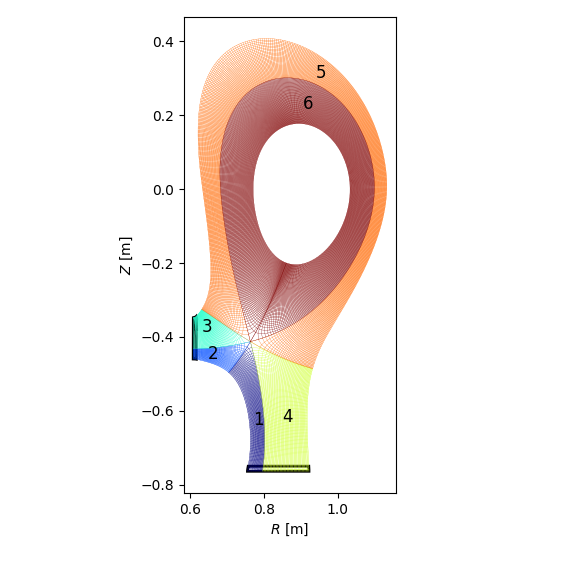
\includegraphics[width=1\textwidth]{schemes/TCVmesh.png}
		\subcaption{Typical mesh and zones decomposition in a poloidal plane of tokamak}
		\label{fig:TCVmesh}
	\end{subfigure}
	\begin{subfigure}[t]{0.3\textwidth}
		\centering
		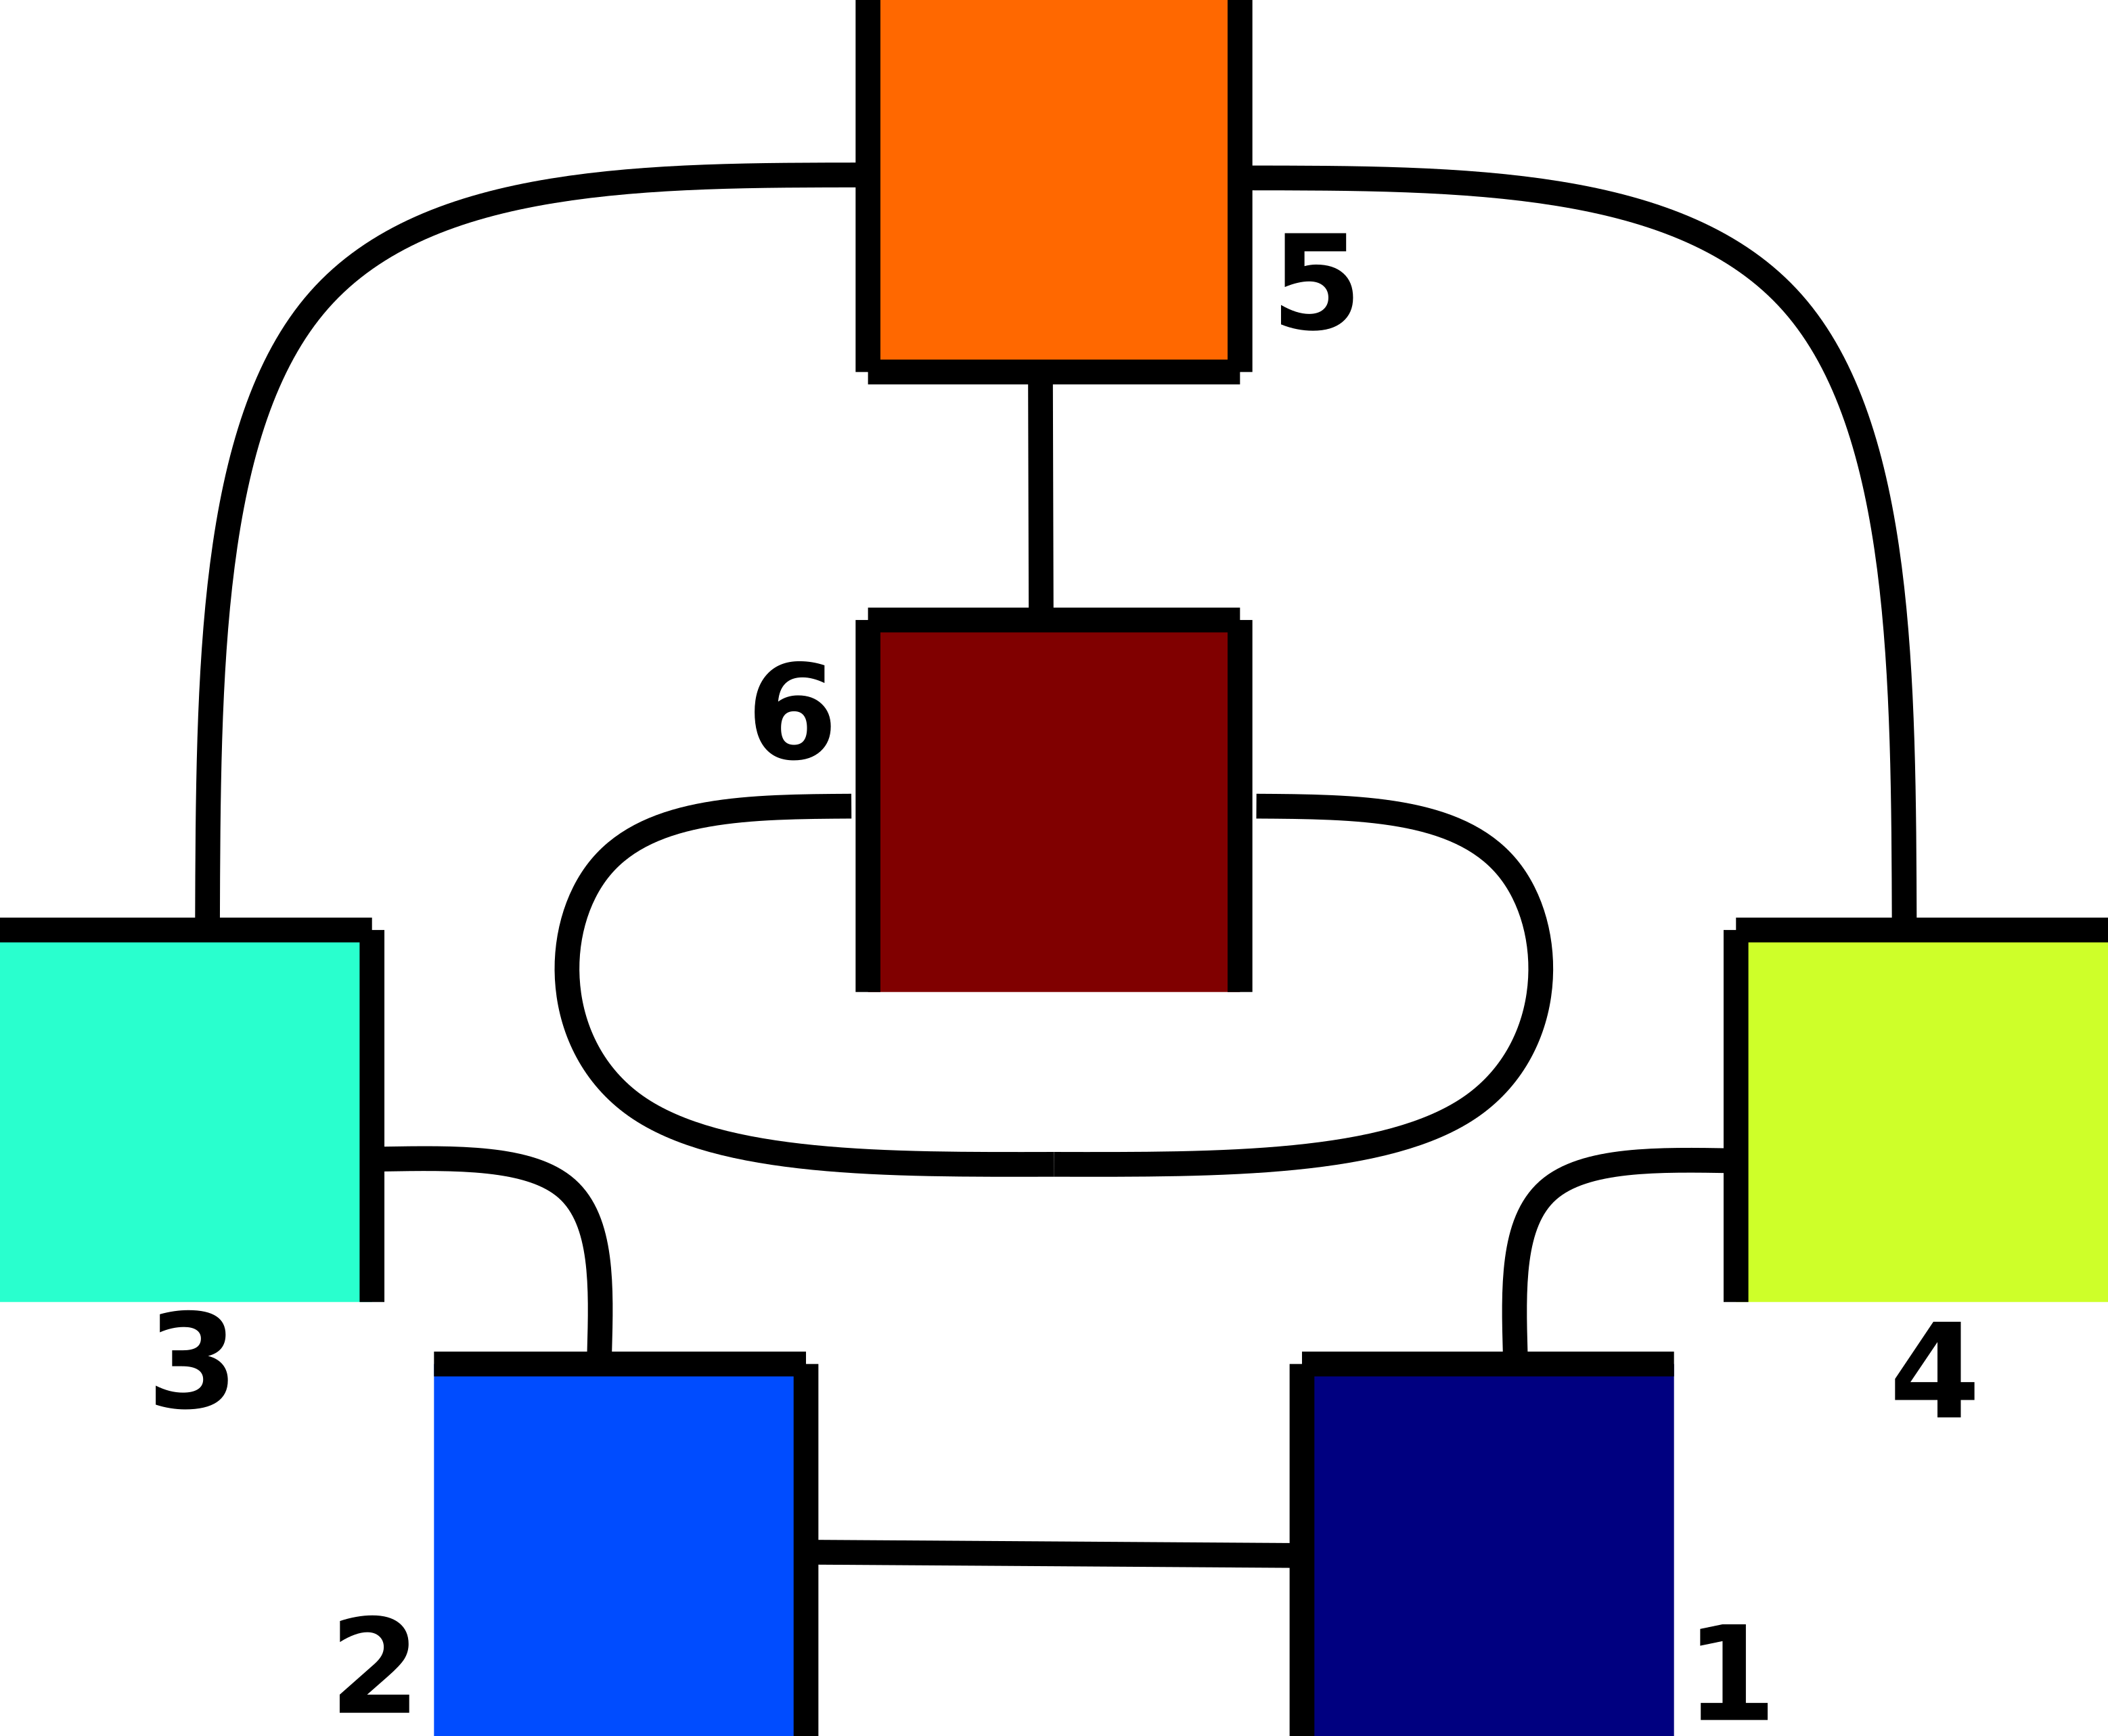
\includegraphics[width=1\textwidth]{schemes/TCV_domains.png}s
		\subcaption{Zones in the domain decomposition}
		\label{fig:TCV_domains}
	\end{subfigure}
	
	\caption{ Example of typical mesh and domain decomposition mapping the real domain (a) to a Cartesian multiple zones domain (b). Each colored zone is isomorphic to a cube, the lines connecting the edges indicate the neighbours mapping. }
	\label{fig:TCVzoneDecomposition}
\end{figure}

\subsection{Curvilinear coordinates}
\label{ssec:MetricCurvilinearCoordinates}
As it was described in the previous \autoref{ssec:SpatialDiscretization}, the spatial discretization involves a curved grid in poloidal $\theta$ and toroidal $\varphi$ directions. The second chapter of the book by D’haeseleer et al \cite{CurvilinearGrids} describes well the numerical implications of curvilinear grids and serves as the basis of the present implementation. \\
Let $U=[u^\psi, u^\theta, u^\varphi]^T$ be the three parameters that describe every point in the domain $\Omega$ with respect to the curvilinear system of coordinates. On a torus, we can find an invertible transformation $R$ that maps each possible $U\in\Omega$ to a unique point in cartesian coordinates, thus: 
$$ \begin{bmatrix} x \\ y \\ z\end{bmatrix} = \vec{R}(u^\psi, u^\theta, u^\varphi) $$
If we fix one parameter and allow the two remaining to vary freely, we obtain the so-called coordinate surface. Analogously if we fix two parameters, we obtain the coordinate curve associated to the free parameter and an accommodating choice for the scalar values $u^i$ is the curve length from an arbitrary reference point. At any point $P\in\Omega$, a local basis ${\vec{e}_\psi, \vec{e}_\theta, \vec{e}_\varphi}$ can be defined by the tangents to the respective coordinate curves crossing this point. Consequently, the basis vectors are easily expressed as:
\begin{align*}
	\vec{e}_\psi =& \pdv{\vec{R}}{u^\psi} & \vec{e}_\theta =& \pdv{\vec{R}}{u^\theta} & \vec{e}_\varphi =& \pdv{\vec{R}}{u^\varphi}
\end{align*}
The parameter choice of $u^i$ can be seen as the curve length and it might or might not be a unit length. The dimension index appears in subscript $\vec{e}_i$ to indicate that the basis vectors originate from a $u^i$ located below the fraction line. \\
An alternative basis can be defined from the gradients of the parameters $u^i$ which hence uses a superscript notation:  
\begin{align*}
	\vec{e}^\psi = & \grad{u^\psi} & \vec{e}^\theta = & \grad{u^\theta} & \vec{e}^\varphi = & \grad{u^\varphi}
\end{align*}
These basis vectors are orthogonal to the respective coordinate surfaces at the point $P$. It can be shown that both basis are reciprocal, thus:
$$ e^i\cdot e_j = \delta^i_j $$
where $\delta^i_j$ is the Kronecker delta. \\
This leads to the introduction of the covariant (linked to subscripts) and contravariant (linked to the superscripts) components of a vector. As it is known from linear algebra, any vector $\vec{v}$ can be expressed with respect to an arbitrary basis $\tilde{\vec{e}_i}$ as $\vec{v}=\tilde{v}_i\tilde{\vec{e}}_i$. For the two previously introduced basis, the respective components of $\vec{v}$ are given by: 
\begin{align*}
	\text{Covariant components: }    & v_i = \vec{v}\cdot\vec{e}_i & \Rightarrow && \vec{v} = v_i\vec{e}^i \\
	\text{Contravariant components: }& v^i = \vec{v}\cdot\vec{e}^i & \Rightarrow && \vec{v} = v^i\vec{e}_i \\
\end{align*}
It is common practice to call the representation of $\vec{v}$ using the co-/contravariant components the co-/contravariant vector of $\vec{v}$ albeit the co- and contravariant vectors both naturally describe the same vector $\vec{v}$. \\
Next, we introduce the metric coefficients $g_{ij} = \vec{e}_i\cdot \vec{e}_j$ and their reciprocal metric coefficients $g^{ij} = \vec{e}^i\cdot \vec{e}^j$. If available, they allow for an easy both-way conversion of contravariant to covariant vectors and consequently an easy change of basis. 
\begin{align*}
	v_i =& g_{ij}v^j & \vec{e}_i =& g_{ij}\vec{e}^j \\
	v^i =& g^{ij}v_j & \vec{e}^i =& g^{ij}\vec{e}_j 
\end{align*}
It may be noted that the matrices formed by the indices $i,j\in\{\theta,\psi,\varphi\}$ are each other's inverse matrix. \\



\subsubsection{Linear algebra}
The metric coefficients together with the co-/contravariant vectors are useful tools to perform several operations on the curvilinear grid. First of all, the squared Jacobian of the transformation from the cartesian to the curvilinear coordinate systems is equal to the determinant of $g_{ij}$. 
\begin{align}
	J = \pdv{(x,y,z)}{(u^\psi, u^\theta, u^\varphi)} = \sqrt{\det\left[g_{ij}\right]} \label{eq:MetricJacobian}
\end{align}
The dot product between two vectors $\vec{v}$ and $\vec{w}$ is calculated with the co-/contravariant vectors.
\begin{align}
	\vec{v}\cdot\vec{w} = g_{ij}v^iw^j = g^{ij}v_iw_j \label{eq:MetricDotProduct}
\end{align}
The co-/contravariant components of the cross product can also be calculated: 
\begin{align}
	\begin{cases}
		(\vec{v} \cross \vec{w})_k = J\epsilon_{ijk}v^iw^j \\
		(\vec{v} \cross \vec{w})^k = \frac{1}{J}\epsilon_{ijk}v_iw_j
	\end{cases} \label{eq:MetricCrossProduct}
\end{align}
This operations involves the Levi-Civita symbol $\epsilon_{ijk}$ which takes the value $+1$ for all even permutations $\{\psi,\theta,\varphi\}$,$\{\theta,\varphi,\psi\}$ and $\{\varphi,\psi,\theta\}$, the value $-1$ for all odd permutations $\{\varphi,\theta,\psi\}$,$\{\theta,\psi,\varphi\}$ and $\{\psi,\varphi,\theta\}$, and is $0$ for all other cases. \\
In various formulae such as ..., ... or ... of the SOLEDGE3X model, we need to split a vector into its parallel and perpendicular component with respect to the magnetic field $\vec{B}$.
\begin{align}
	\vec{v}_\parallel &= \vec{v}\cdot\vec{b} & \vec{v}_\perp &= -\vec{b}\cross (\vec{b}\cross\vec{v}) \label{eq:MetricParalPerpVecComponents}
\end{align}
The vector $\vec{b}$ contains the normalized magnetic field and hence represents a unit vector in parallel direction at each point. In the code only its co- and contravariants are calculated and stored for the entire mesh: 
\begin{align}
	b_\psi &= \vec{b} \cdot \vec{e}_\psi & b_\theta &= \vec{b} \cdot \vec{e}_\theta & b_\varphi &= \vec{b} \cdot \vec{e}_\varphi \label{eq:MetricCovariantUnitB} \\
	b^\psi &= \vec{b} \cdot \vec{e}^\psi & b^\theta &= \vec{b} \cdot \vec{e}^\theta & b^\varphi &= \vec{b} \cdot \vec{e}^\varphi \label{eq:MetricContravariantUnitB}
\end{align} 


\subsubsection{Differentiation}
The gradient of a scalar field $S(u^\psi, u^\theta, u^\varphi)$ is calculated in terms of the reciprocal basis: 
\begin{align}
	\left(\grad{S}\right)_i = \pdv{S}{u^i}\vec{e}^i \label{eq:MetricGradient}
\end{align}
In the transport equations, we need to calculate gradients in parallel direction of the field which allows us to express $\vec{\grad}_\parallel$ in terms of the contravariant vector of the unit magnetic field from \autoref{eq:MetricContravariantUnitB}.
\begin{align}
	\grad_\parallel S = \pdv{S}{u^i}\vec{b}\cdot\vec{e}^i = \pdv{S}{u^\theta}b^\theta + \pdv{S}{u^\varphi}b^\varphi \label{eq:MetricParallelGradient}
\end{align}
The terms in $\psi$ are omitted in the above formula since the equilibrium magnetic flux surfaces are located on the $\theta$-$\varphi$ coordinate surface and the vector $\vec{b}$ has therefore a zero value in its radial component. Note that this gradient is a scalar as it always points in $\vec{b}$ direction. \\
Similarly, a perpendicular gradient can be defined as: 
\begin{equation*}
	\vec{\grad}_\perp S = \vec{\grad} S - \left(\grad_\parallel S\right)\vec{b}
\end{equation*}
In terms of metric coefficients, it translates to: 
\begin{align}
	\label{eq:MetricPerpendicularGradient}
	\left(\vec{\grad}_\perp S\right)^i =& g^{ij}\left(\grad{S}\right)_j - \left(\grad_\parallel S\right)b^i \nonumber \\
	=& g^{ij}\pdv{S}{u^j} - \left(\pdv{S}{u^\theta}b^\theta + \pdv{S}{u^\varphi}b^\varphi\right)b^i
\end{align}
We have to keep in mind that the above expression leads to the contravariant components of the perpendicular gradient whereas the general expression for the gradient in \autoref{eq:MetricGradient} gives its covariant components. \\

Next, the divergence of a vector $\vec{v}$ is calculated by: 
\begin{align}
	\vec{\grad}\cdot\vec{v} = \frac{1}{J}\pdv{(JA^i)}{u^i} \label{eq:MetricDivergence}
\end{align}

and further the divergence of parallel vector fields $S_\parallel\vec{b}$ comes in handy: 
\begin{align}
	\vec{\grad}\cdot \left(S_\parallel\vec{b}\right) = \frac{1}{J}\left[\pdv{\left(J S_\parallel b^\theta\right)}{u^\theta} + \pdv{\left(J S_\parallel b^\varphi\right)}{u^\varphi}\right] \label{eq:MetricDivergenceParallel}
\end{align}

The gradient and divergence operators can be combined o define a diffusion operator. The parallel Laplacian with some diffusion coefficients $D$ reads in metric terms: 
\begin{align}
	\label{eq:MetricParallelDiffusion}
	\vec{\grad}\cdot\left[D\left(\grad_\parallel S\right)\vec{b}\right] = \frac{1}{J}\left[\pdv{\left(JD \left(\pdv{S}{u^\theta}b^\theta + \pdv{S}{u^\varphi}b^\varphi\right) b^\theta\right)}{u^\theta} + \pdv{\left(JD\left(\pdv{S}{u^\theta}b^\theta + \pdv{S}{u^\varphi}b^\varphi\right) b^\varphi\right)}{u^\varphi}\right]
\end{align}

Similarly, a perpendicular diffusion operator can be defined: 
\begin{align}
	\vec{\grad}\cdot\left[D\vec{\grad}_\perp S\right] =& \vec{\grad}\cdot\left[D\left(\vec{\grad} S - \left(\grad_\parallel S\right)\vec{b}\right)\right] \nonumber \\
	=& \frac{1}{J}\pdv{}{u^i}\left[JD\left(g^{ij}\pdv{S}{u^j} - \left(\pdv{S}{u^\theta}b^\theta + \pdv{S}{u^\varphi}b^\varphi\right)b^i\right)\right] \nonumber \\
	=& \frac{1}{J}\left(\pdv{}{u^\psi}\left[JD\left(g^{\psi\psi}\pdv{S}{u^\psi} + g^{\psi\varphi}\pdv{S}{u^\theta} + g^{\psi\theta}\pdv{S}{u^\varphi}\right)\right]      \right.\nonumber \\
	&+ \pdv{}{u^\theta}\left[JD\left(g^{\theta\psi}\pdv{S}{u^\psi} + \left(g^{\theta\theta} - b^\theta b^\theta\right)\pdv{S}{u^\theta} + \left(g^{\theta\varphi} - b^\varphi b^\theta\right)\pdv{S}{u^\varphi}\right)\right] \nonumber \\
	&+ \left. \pdv{}{u^\varphi}\left[JD\left(g^{\varphi\psi}\pdv{S}{u^\psi} + \left(g^{\varphi\varphi} - b^\theta b^\varphi\right)\pdv{S}{u^\theta} + \left(g^{\varphi\theta} - b^\varphi b^\varphi\right)\pdv{S}{u^\varphi}\right)\right]\right) \label{eq:MetricPerpendicularDiffusion}
\end{align}

\subsection{Finite volume approach}

The spatial discretization is based on a second-order conservative finite-volume scheme associated with a 3rd-order WENO reconstruction and Donat, Marquina fluxes for a modified Riemann solver for the advection terms to handle both shocks and complicated smooth solution structures \cite{tamain2016tokam3x, Bufferand2021}. \newline




\section{The staggered mesh}

In order to benefit from the first-order parallel derivative that separates the $A_\parallel$ and $j_\parallel$ from the other plasma fields $\Phi$, $n_e$, and $T_e$ (Eqs. \ref{eq:MagneticPotential} and \ref{eq:VorticityEquation}), these two variables are defined on a toroidally $\varphi$ and poloidally $\theta$ staggered grid. They are calculated at cell edges in the parallel direction and can be directly matched to the fluxes entering and leaving the collocated cells. One of the major benefits is to minimize numerical diffusion and preserve turbulent structures, following findings in FVM simulations for fluid mechanics \cite{meier1999comparison}. In the radial $\psi$ direction, we keep the collocated position as the only parallel gradient in $\psi$ comes from the flutter term, which in nature is much smaller than the equilibrium field. If the mesh were also staggered in $\psi$, we would face strong numerical radial diffusion of parallel fluxes, defying the motivation of a staggered grid for $A_\parallel$ and $j_\parallel$. \newline


\subsection{Description and notation of the staggered grid}
The scalar variable $A_\parallel$ is the magnitude of the parallel magnetic vector potential that is a factor of the unit vector $\vec{b}$ in direction of the externally induced magnetic field lines. By construction of the domain, $\vec{b}$ has only components in $\varphi$ and $\theta$ directions. So far, all physical quantities are calculated on the collocated grid points at the domain cell centers. In the newly introduced equation on $A_\parallel$, the magnetic vector potential appears homogeneous to the potential, pressure and temperature gradients and the additional $A_\parallel$ term in the original equation states that the divergence of $A_\parallel$ accounts for the change in vorticity. Thus, $A_\parallel$ is always one spatial derivative away from the original quantities. As it is common in classical CFD simulation the velocity, $A_\parallel$ is not defined on cell centers but on a staggered grid on the cell edges in $\psi$-direction. Because the magnetic field lines do not evolve in radial direction and only parallel gradients contribute to $A_\parallel$, its grid is only staggered in  poloidal and toroidal directions. To distinguish quantities on both grids, the indexes $[i_\psi, i_\theta - \frac{1}{2},i_\varphi-\frac{1}{2}]$ describe discrete positions on the staggered grid. \\

\begin{figure}[H]
	\centering
	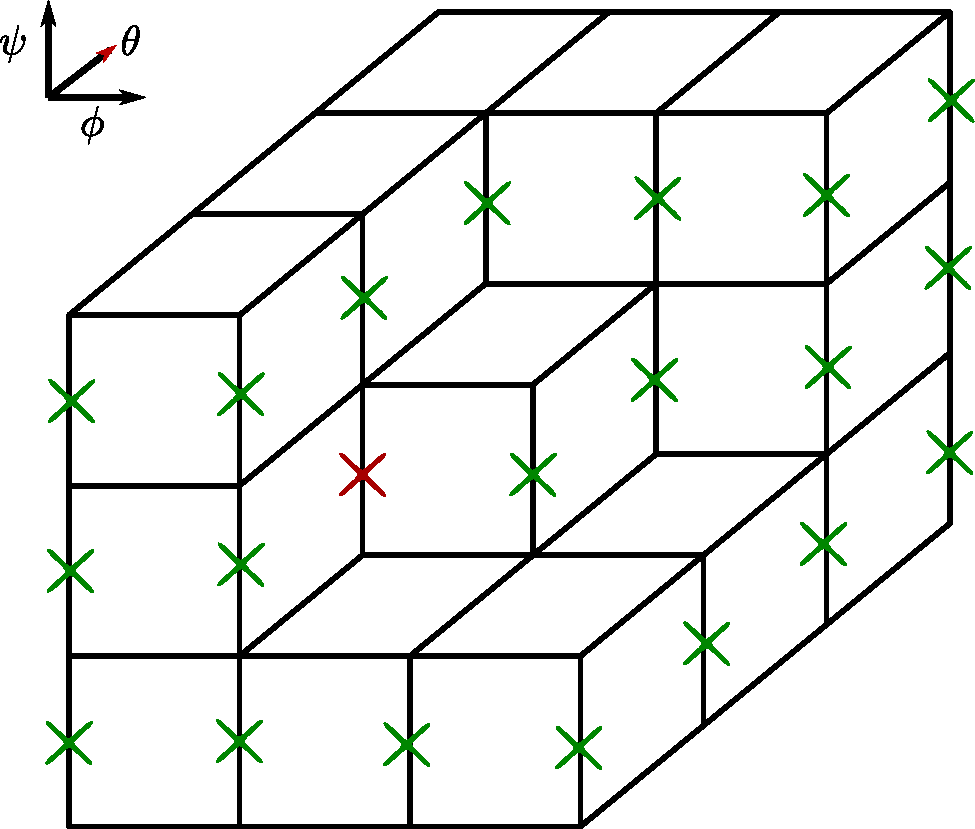
\includegraphics[width=0.4\textwidth]{schemes/StaggeredGrid.pdf}
	\caption{General view of the staggered grid points marked as crosses on top of the collocated cells. The red cross at the position $[i_\psi, i_\theta - \frac{1}{2}, i_\varphi-\frac{1}{2}]$ corresponds to the central cell with index $[i_\psi, i_\theta, i_\varphi]$}
	\label{fig:StaggeredGridOverview}
\end{figure}

In the following work, quantities evaluated at staggered grid points are indicated either by the superscript $stg$ or by a $-\frac{1}{2}$ shift in the index. This means that following notations are equivalent: 
\begin{align*}
	X^{stg}_{[i_\psi,i_\theta,i_\varphi]} &= X_{[i_\psi,i_\theta-\frac{1}{2},i_\varphi-\frac{1}{2}]} &\text{or}&& X^{stg}_{[i_\psi,i_\theta+1,i_\varphi]} &= X_{[i_\psi,i_\theta+\frac{1}{2},i_\varphi-\frac{1}{2}]}
\end{align*}

\subsection{Boundary cells}

Staggered quantities require a different treatment at the domain boundary. In the geometry definition, entire cells belong either to the plasma or to the physical wall. Collocated quantities in the boundary layer are thus always half a cell width away from the wall and boundary conditions are enforced accordingly. For the magnetic vector potential this holds for walls in $\psi$ direction but in $\varphi$ and $\theta$ directions, the staggered grid points are on the tokamak wall for the boundary cells with lowest index and one cell width away at the highest index. For consistency, accuracy and symmetry purposes, the staggered solvable domain shall be either extended by one row of cells at the upper index to include the wall in the solution or or reduced by one row at the lower end. In both cases, the number of collocated and staggered grid points do not match anymore and inhibit all eventual symmetry properties of the matrix in the dual-grid system (\ref{eq:vorticityEquation_electromagnetic_dedimensionalized_implicitEulerSystem}). $A_\parallel$ requires Dirichlet boundary conditions with the value 0 everywhere, thus the solution on the wall is already known and is not needed in the system. Therefore the latter option without the staggered grid points of the lower boundary cell layer is more suitable and has been implemented as depicted in \autoref{fig:StaggeredGridBC}.
\begin{figure}[H]
	\centering
	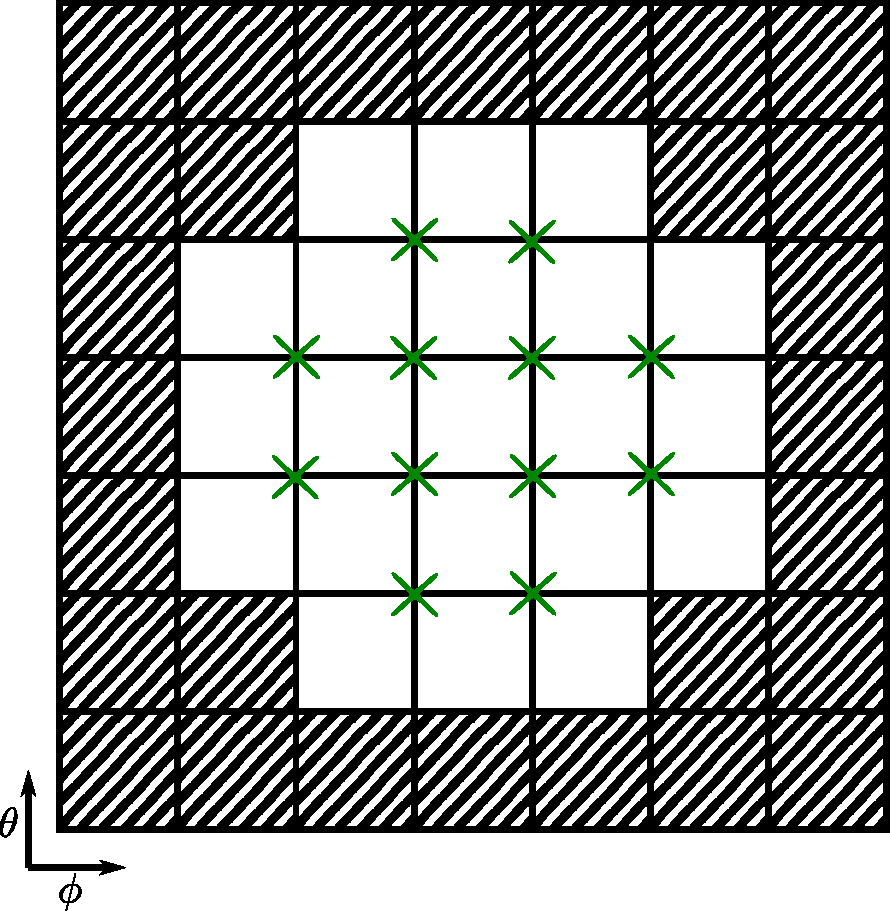
\includegraphics[width=0.4\textwidth]{schemes/staggeredGridBoundary.pdf}
	\caption{General view of the staggered grid points in the $\theta-\varphi$ plane that are solved in the vorticity equation. Note that at the lower boundaries, collocated fields are included in the system but not their staggered counterparts. }
	\label{fig:StaggeredGridBC}
\end{figure}
In the system (\ref{eq:vorticityEquation_electromagnetic_dedimensionalized_implicitEulerSystem}), some entries for the electric potential $\Phi$ do not have a corresponding magnetic potential $A_\parallel$. To ensure a correct implementation of the system and the stencils that appear in it, a new mask $\chi^{stg}$ describes which cells contain staggered grid points in the solvable domain. It is defined from the original collocated wall mask $\chi$ as: 
\begin{equation}
	\label{eq:def_chi_staggered}
	\chi^{stg}_{[i_\psi,i_\theta, i_\varphi]} = 1 - (1 - \chi_{[i_\psi,i_\theta  ,i_\varphi  ]})
	(1 - \chi_{[i_\psi,i_\theta-1,i_\varphi  ]})
	(1 - \chi_{[i_\psi,i_\theta  ,i_\varphi-1]})
	(1 - \chi_{[i_\psi,i_\theta-1,i_\varphi-1]})
\end{equation}
The value of $\chi^{stg}_{[i_\psi,i_\varphi,i_\theta]}$ is therefore 1 if the staggered grid point of the cell with index $[i_\psi,i_\varphi,i_\theta]$ lies on or in the wall and it is 0 inside the solvable domain.



Another implication for staggered fields occurs at sheath boundaries, where $A_\parallel$ and $j_\parallel$ lie on the domain boundary. For collocated fields, we impose sheath fluxes from the Bohm-Chodura model (see Sec. \ref{sec:boundaryConditions}) on the first cell in the simulation domain. For the magnetic potential $A_\parallel$, the 0-Dirichlet condition is imposed in the concerned cell. For the parallel current $j_\parallel$, we add the sheath current $j_{\text{wall}}$ to any parallel currents tangential to the wall. Indeed, if the sheath boundary is in the $\theta$ direction, the $\varphi$ component of the parallel current remains unaffected and needs to be solved. 



\subsection{Staggered discrete operators}
As the parallel current $j_\parallel$ and the magnetic vector potential $A_\parallel$ are defined on a staggered grid, new stencil operators are needed to be compatible with the electric potential $\Phi$ defined on the collocated grid at the cell centers. 

\subsubsection{Divergence on a parallel vector field}

In \autoref{eq:vorticityEquation_electromagnetic}, the divergence of $j_\parallel$ needs to be calculated at the collocated grid. We thus need a discrete stencil operator 
$$\left[\grad\cdot X^{stg}\vec{b}\right]^{col}_{[i_\psi,i_\theta, i_\varphi]}$$
In \autoref{eq:MetricDivergenceParallel}, the divergence of a parallel vector field has been introduced. We consider a collocated cell as in \autoref{fig:StaggeredGridOverview}. The flux $\pdv{\left(J X b^\theta\right)}{u^\theta}$ is then the difference between the inflow and the outflow through the two cell faces facing the $\theta$ axis. We want to calculate these fluxes from the flux $F^{X,in} = JXb^\theta$ of the staggered field $X$ known at the crosses in the schematic. We further assume that the inflow to the central collocated cell is the mean of the fluxes at the red cross and at the green cross right to it:
\begin{align*}
	F_{[i_\psi,i_\theta, i_\varphi]}^{X,\theta} &= \frac{1}{2}\left(F_{[i_\psi,i_\theta-\frac{1}{2}, i_\varphi-\frac{1}{2}]}^{X,\theta} + F_{[i_\psi,i_\theta-\frac{1}{2}, i_\varphi+\frac{1}{2}]}^{X,\theta} \right) \\
	&= J_{[i_\psi,i_\theta-\frac{1}{2}, i_\varphi-\frac{1}{2}]}X_{[i_\psi,i_\theta-\frac{1}{2}, i_\varphi-\frac{1}{2}]}b_{[i_\psi,i_\theta-\frac{1}{2}, i_\varphi-\frac{1}{2}]}^\theta + J_{[i_\psi,i_\theta-\frac{1}{2}, i_\varphi+\frac{1}{2}]}X_{[i_\psi,i_\theta-\frac{1}{2}, i_\varphi+\frac{1}{2}]}b_{[i_\psi,i_\theta-\frac{1}{2}, i_\varphi+\frac{1}{2}]}^\theta
\end{align*}

If one of the two staggered points lies on the domain boundary, it is not included in the flux calculation and consequently the factor $1/2$ is dropped. \\

This numerical calculation can be performed for all in- and outflows in $\theta$ and $\varphi$ directions, leading to the final form of the numerical form of the staggered divergence stencil: 
\begin{equation}
	\label{eq:NumericalStaggeredDivergenceStencil}
	\left[\grad\cdot X^{stg}\vec{b}\right]^{col}_{[i_\psi,i_\theta, i_\varphi]} = \frac{1}{J_{[i_\psi,i_\theta, i_\varphi]}} \left(F_{[i_\psi,i_\theta, i_\varphi]}^{X,\theta}-F_{[i_\psi,i_\theta+1, i_\varphi]}^{X,\theta}+F_{[i_\psi,i_\theta, i_\varphi]}^{X,\varphi}-F_{[i_\psi,i_\theta, i_\varphi+1]}^{X,\varphi}\right)
\end{equation}

\subsubsection{Parallel gradient}

In \autoref{eq:vorticityEquation_electromagnetic}, another operator is needed to represent the gradient of $A_\parallel \vec{b}$ on the staggered grid.
$$\left[\grad_\parallel X^{col}\right]^{stg}_{[i_\psi,i_\theta, i_\varphi]}$$
According to \autoref{eq:MetricParallelGradient}, its numerical evaluation is quite straight-forward: 
\begin{align}
	\label{eq:NumericalStaggeredParallelGradientStencil}
	\left[\grad_\parallel X^{col}\right]^{stg}_{[i_\psi,i_\theta, i_\varphi]} =& \frac{1}{2}\left(X_{[i_\psi,i_\theta, i_\varphi]}-X_{[i_\psi,i_\theta-1, i_\varphi]}\right)b_{[i_\psi,i_\theta-\frac{1}{2}, i_\varphi-\frac{1}{2}]}^\theta \nonumber \\ +& 
	\frac{1}{2}\left(X_{[i_\psi,i_\theta, i_\varphi]}-X_{[i_\psi,i_\theta, i_\varphi-1]}\right)b_{[i_\psi,i_\theta-\frac{1}{2}, i_\varphi-\frac{1}{2}]}^\varphi
\end{align}

If any of the used $X$ happens to lie inside the boundary, it is eliminated from the stencil. \\

The staggered divergence and parallel gradient stencils already existed in a hidden form in the original SOLEDGE implementation as part of the parallel Laplacian operator on collocated fields, which first computes the parallel gradient leading to intermediate staggered results and then applies the divergence operator on these staggered intermediate results.

\subsubsection{Perpendicular Laplacian}

Finally, \autoref{eq:vorticityEquation_electromagnetic} requires the perpendicular Laplacian on the staggered grid to link $j_\parallel$ and $A_\parallel$.

$$\left[\Delta_{\perp}X^{stg}\right]^{stg}_{[i_\psi,i_\theta, i_\varphi]}$$

In the scheme proposed by G\"{u}nter et al. \cite{Gnter2005ModellingOH}, this operation is performed in two steps: first the perpendicular gradient is evaluated on $X^{stg}$ which produces an intermediate collocated vector field $\vec{Y}^{col}$ whose divergence leads to the final staggered result. \autoref{eq:MetricPerpendicularDiffusion} includes all needed metrics to achieve this operation. To better understand the final divergence operation, we must imagine a cell centered around the point where the perpendicular Laplacian is required, depicted in \autoref{fig:StaggeredCell}. We then need to calculate the fluxes $F^{Y,i}$ across all six faces. The metric and diffusion coefficients $JD(g^{ij}-b^ib^j)$ are also required at the faces and we obtain them by taking their average on the closest collocated points. In poloidal and toroidal directions two collocated points shown in green in \autoref{fig:StaggeredFluxTheta} and \autoref{fig:StaggeredFluxPhi} are sufficient but in radial direction we need to consider eight points around the face to calculate the correct coefficients. \\

\begin{figure}[H]
	\centering
	\begin{subfigure}[b]{0.24\textwidth}
		\centering
		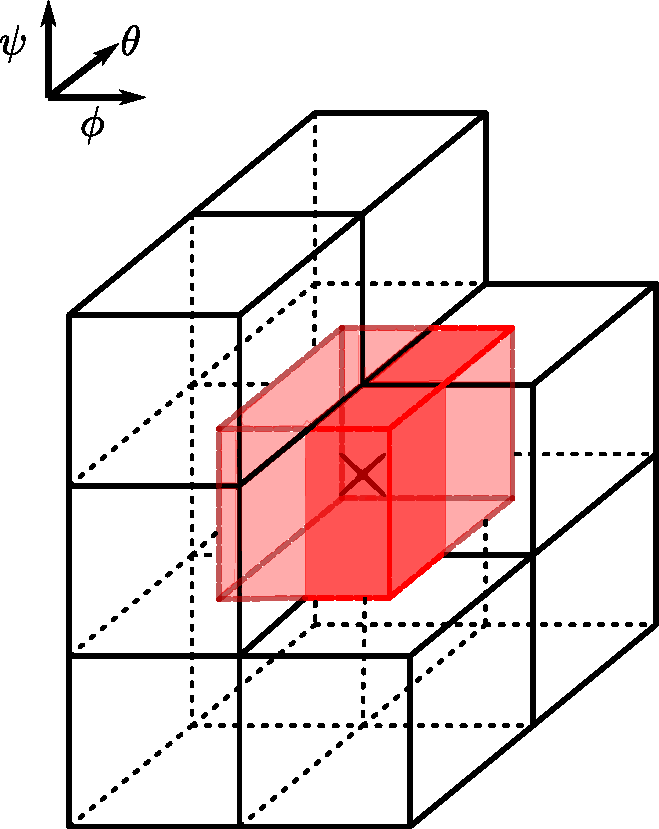
\includegraphics[width=1\textwidth]{schemes/BoundingBoxStaggeredPoint.pdf}
		\subcaption{Cell boundaries \\ for the staggered \\ grid point}
		\label{fig:StaggeredCell}
	\end{subfigure}
	\begin{subfigure}[b]{0.24\textwidth}
		\centering
		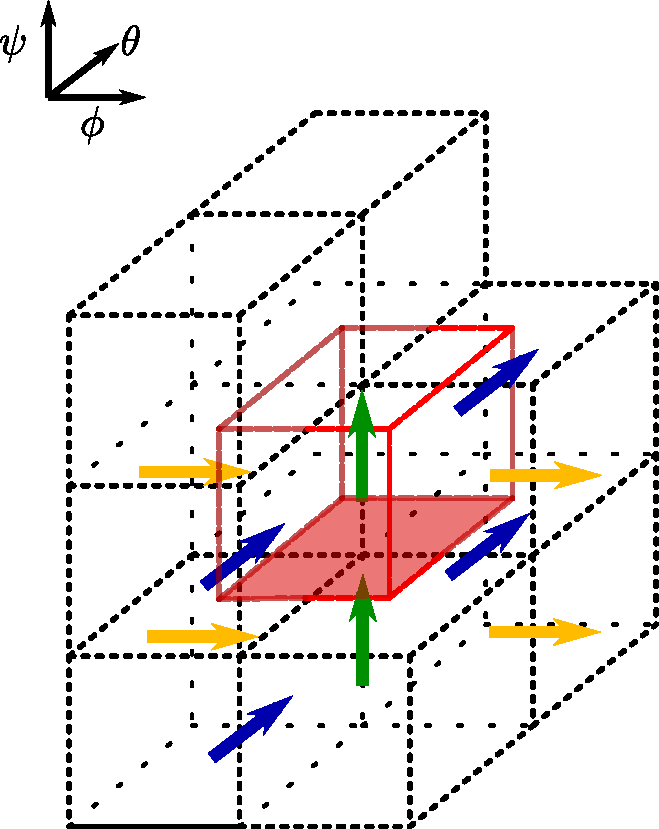
\includegraphics[width=1\textwidth]{schemes/BoundingBoxFluxPsiDiffPerp.pdf}
		\subcaption{Relevant faces \\ for the outflow face \\ in $\psi$-direction} 
		\label{fig:StaggeredFluxPsi}
	\end{subfigure}
	\begin{subfigure}[b]{0.24\textwidth}
		\centering
		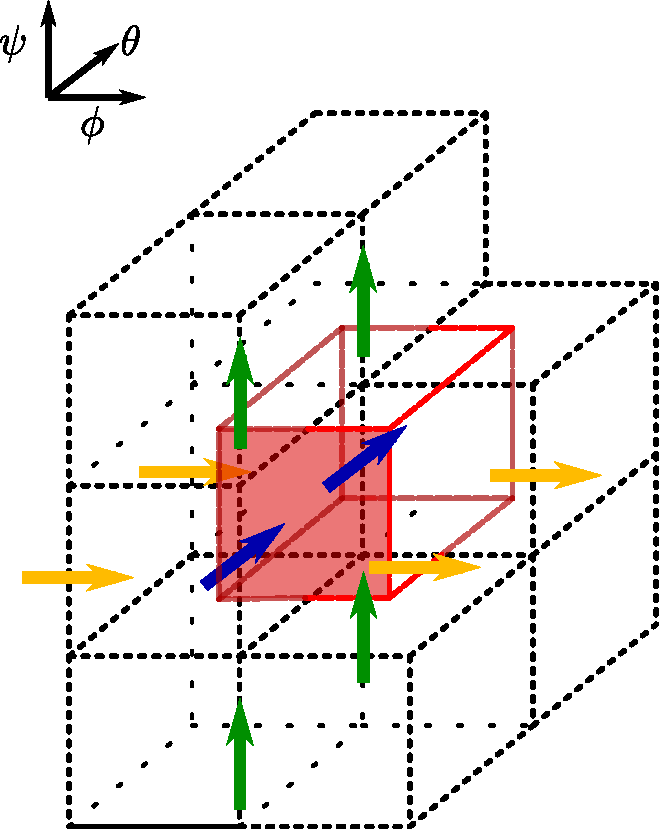
\includegraphics[width=1\textwidth]{schemes/BoundingBoxFluxThetaDiffPerp.pdf}
		\subcaption{Relevant faces \\ for the outflow face \\ in $\theta$-direction} 
		\label{fig:StaggeredFluxTheta}
	\end{subfigure}
	\begin{subfigure}[b]{0.24\textwidth}
		\centering
		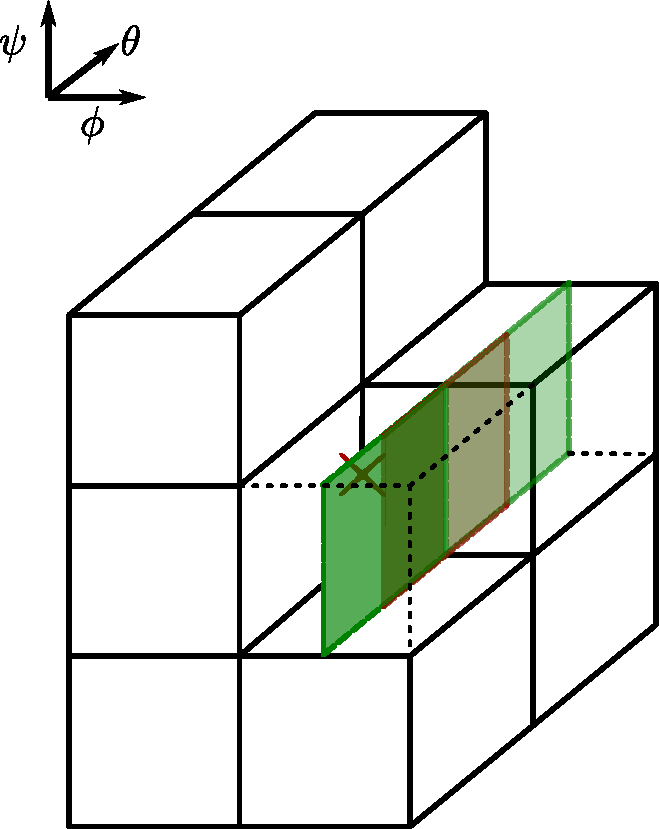
\includegraphics[width=1\textwidth]{schemes/BoundingBoxFluxPhiDiffPerp.pdf}
		\subcaption{Relevant faces \\ for the outflow face \\ in $\varphi$-direction} 
		\label{fig:StaggeredFluxPhi}
	\end{subfigure}
	
	\caption{Depiction of the relevant cell faces to calculate fluxes of a staggered field at coordinate index $[i_\psi, i_\theta-\frac{1}{2}, i_\varphi-\frac{1}{2}]$}
	\label{fig:StaggeredPerpendicularLaplancianCellSurfaces}
\end{figure}

The perpendicular Laplacian can thus be succintly written in term of the fluxes in and out of the staggered red cell:
\begin{align}
	\left[\Delta_{\perp}X^{stg}\right]^{stg}_{[i_\psi,i_\theta, i_\varphi]} =& \frac{1}{J_{[i_\psi,i_\theta-\frac{1}{2}, i_\varphi-\frac{1}{2}]}}\left(F^{Y,\psi}_{[i_\psi+\frac{1}{2},i_\theta-\frac{1}{2}, i_\varphi-\frac{1}{2}]} - F^{Y,\psi}_{[i_\psi-\frac{1}{2},i_\theta-\frac{1}{2}, i_\varphi-\frac{1}{2}]}\right. \nonumber \\ 
	&\left.+ F^{Y,\theta}_{[i_\psi,i_\theta, i_\varphi-\frac{1}{2}]} - F^{Y,\theta}_{[i_\psi,i_\theta-1, i_\varphi-\frac{1}{2}]}+ F^{Y,\varphi}_{[i_\psi,i_\theta-\frac{1}{2}, i_\varphi]} - F^{Y,\varphi}_{[i_\psi,i_\theta-\frac{1}{2}, i_\varphi-1]}\right) 	\label{eq:NumericalStaggeredPerpDiffStencil}	
\end{align}

If any of the staggered cell faces touches the domain boundary in any form, the corresponding flux is excluded from the divergence operator. It only remains to calculate the fluxes $F^{Y,i}$. The metric and diffusion coefficients at all faces have already been described and are represented by the term $\xi^{ij}=JD(g^{ij}-b^ib^j)$. We then can express the fluxes as: 
$$ F^{Y,i} = \xi^{ij}\pdv{X}{u^j} $$
The remaining gradient must use $X^{stg}$ at staggered points in the domain. If $[ijk]$ stands for any permutation of the staggered indices $[i_\psi,i_\theta-\frac{1}{2},i_\varphi-\frac{1}{2}]$ we always have a flux of the kind:
\begin{align*}
	F^{Y,i}_{i-\frac{1}{2},jk} &= \xi^{ii}\left(X^{stg}_{ijk}-X^{stg}_{i-1,jk}\right) \\
	&+ \frac{1}{4}\xi^{ij}\left(X^{stg}_{i,j+1,k}-X^{stg}_{i,j-1,k}+X^{stg}_{i-1,j+1,k}-X^{stg}_{i-1,j-1,k}\right) \\
	&+ \frac{1}{4}\xi^{ik}\left(X^{stg}_{i,j,k+1}-X^{stg}_{i,j,k-1}+X^{stg}_{i-1,j,k+1}-X^{stg}_{i-1,j,k-1}\right)
\end{align*}

If any of the field points $X$ lie in or on the domain boundary, it is not considered in the stencil and the factor $\frac{1}{4}$ is changed to $\frac{1}{3}$.

\subsection{Discretization around the X-point}
\label{ssec:DiscretizationXPt}

The staggered grid has direct implications on the estimation of fluxes around mesh singularities: while for regular fields, every cell around the X-point has well-defined neighbors (see Fig. \ref{fig:CenteredXpoint}), radial fluxes in and out of staggered cells directly cross the X-point (see Fig. \ref{fig:StaggeredXpoint}). They affect the perpendicular Laplacian operator on $A_\parallel$ in Ampere's law (Eq. \ref{eq:MagneticPotential}), advection on $j_\parallel$ in Eq. \ref{eq:advectionJpara}, and the anomalous perpendicular diffusion $\mathcal{D}_\perp$. To cope with the ill-defined cell faces, fluxes across the X-point are forced to 0 by Neumann-like boundary conditions. Neighbors of the involved cells must be defined separately from the regular cells with the same index. \newline

\begin{figure}[H]
	\centering
	\begin{subfigure}[t]{0.39\textwidth}
		\centering
		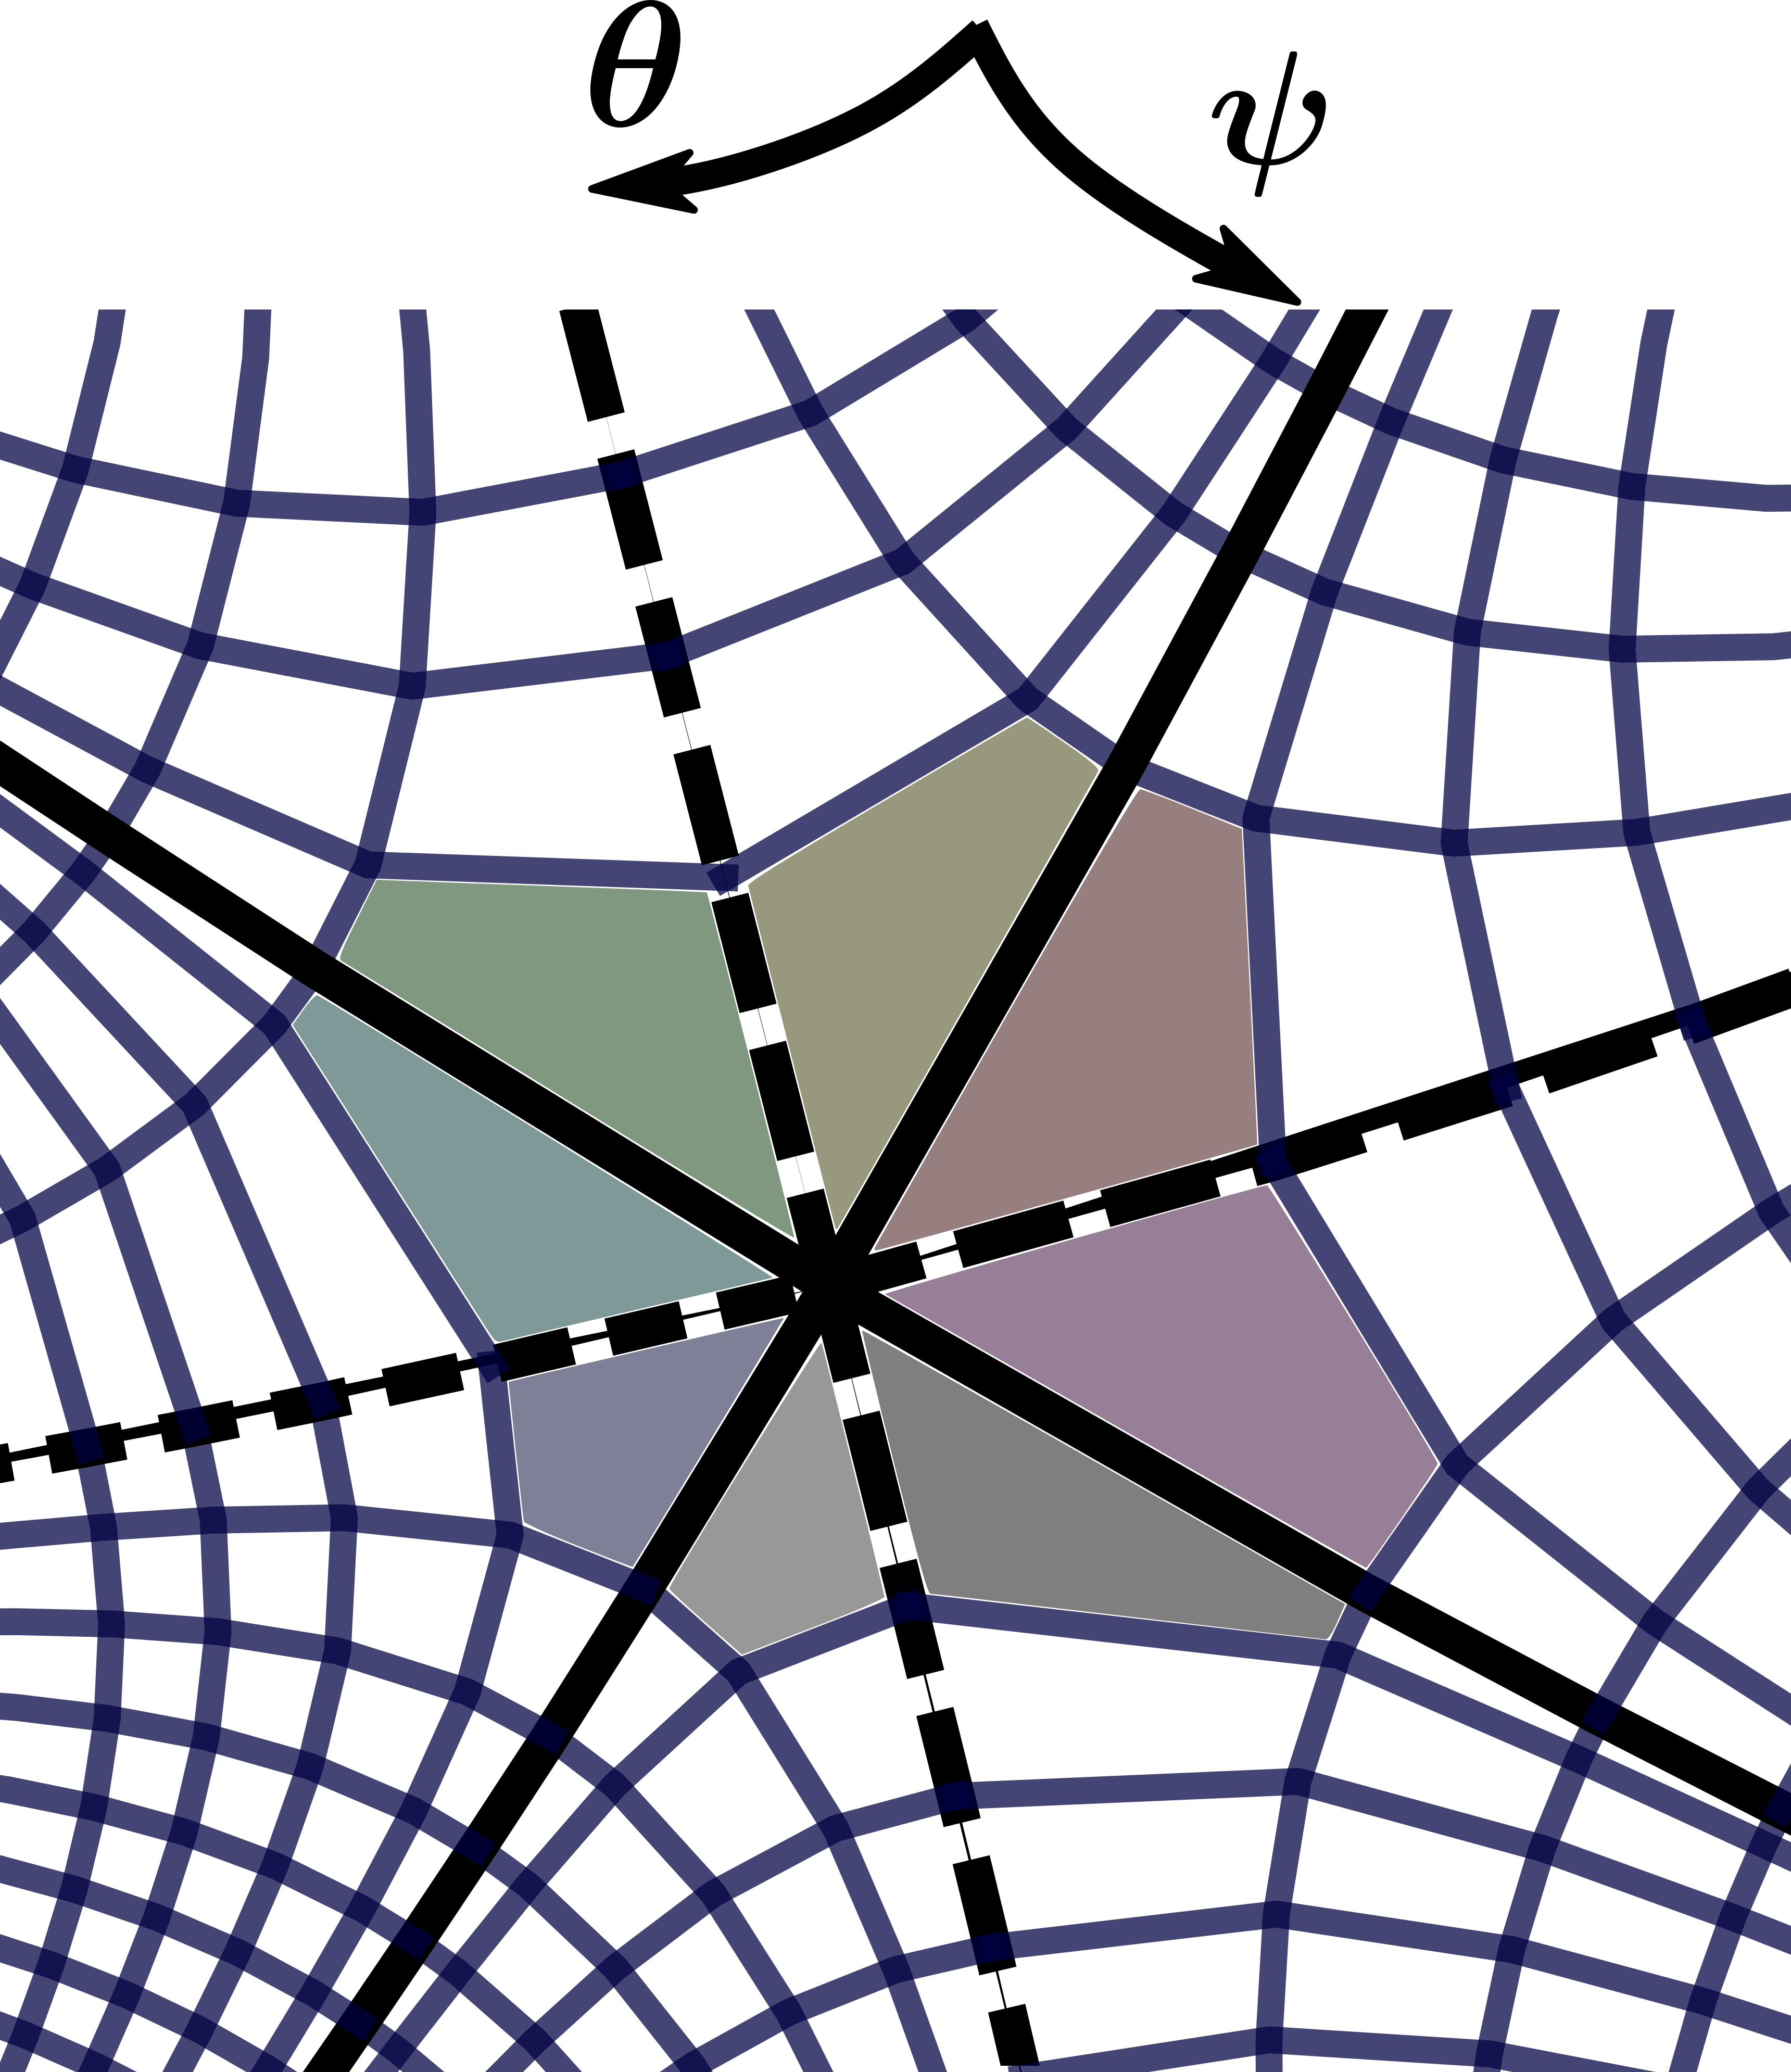
\includegraphics[width=1\textwidth]{schemes/XpointCentered.png}
		\subcaption{View of centered cells}
		\label{fig:CenteredXpoint}
	\end{subfigure}
	\begin{subfigure}[t]{0.39\textwidth}
		\centering
		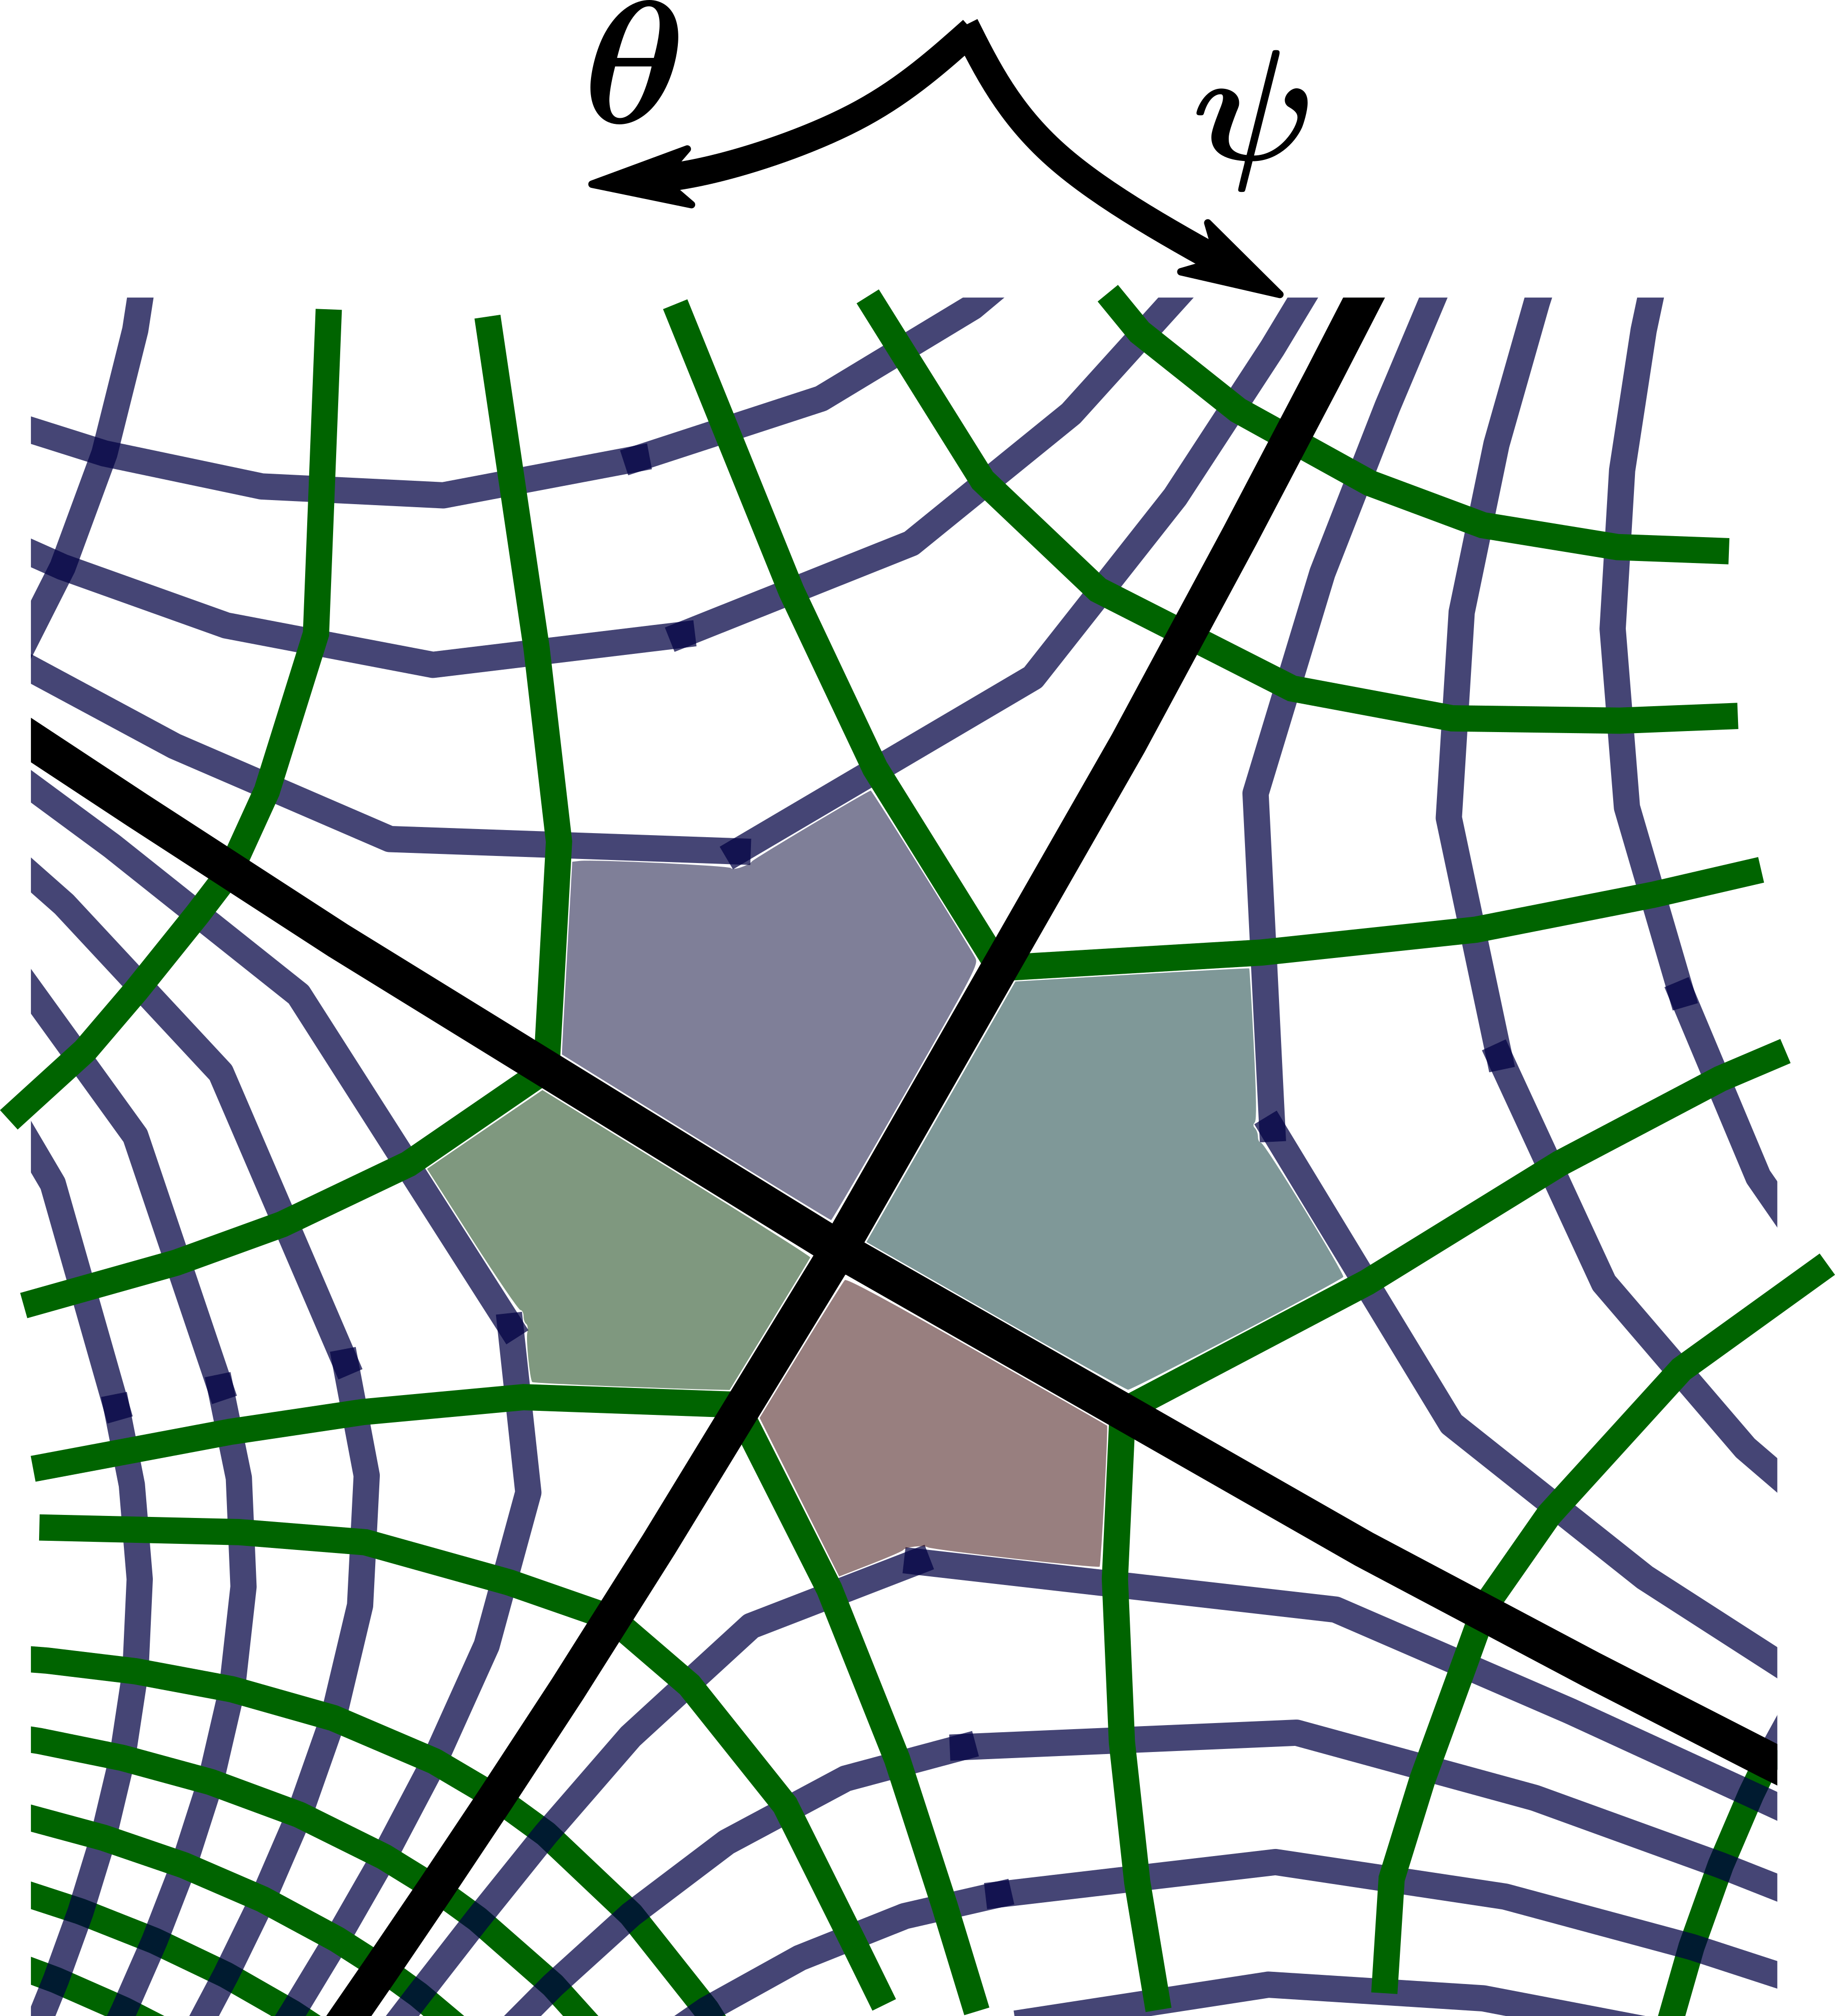
\includegraphics[width=1\textwidth]{schemes/XpointStaggered.png}
		\subcaption{View of staggered cells}
		\label{fig:StaggeredXpoint}
	\end{subfigure}
	\caption{ Sketches of the mesh around the X-point. For centered cells (a), 8 cells touch the X-point at a corner. For staggered cells (b), the X-point is located at the radial face of 4 cells, effectively modifying the shape of the cells to pentagons. Fluxes across the involved faces are hence ill-defined. }
	\label{fig:XpointDiscretization}
\end{figure}



\section{Time discretization}

The model uses an explicit time discretization for the advection terms and an implicit one for the diffusive terms. In turbulence simulations, we limit ourselves to timescales slower than the cyclotronic frequency $\omega_C$. This applies to all advection phenomena, as well as to friction, pressure, and energy source terms, which can then comfortably be solved explicitly in time. \newline

However, ionization/recombination processes, resistive and viscous effects from the Spitzer-Härm model, and electron inertia involve much faster dynamics that would massively constrain the allowed timestep size. Therefore, these terms are solved implicitly. To reduce numerical complexity, they can be decoupled and solved sequentially for the density, the parallel velocity, the temperature, and finally the potentials. 

\subsection{Explicit Runge-Kutta solver}

%Unlike the advection terms, the update of the electric potential in the vorticity equation \ref{eq:ElectrostaticVorticityEquation} requires an implicit numerical scheme, for which we use the 1-st order implicit Euler method. The electric potential $\Phi^{n+1}$ at the next time integration step $n+1$ is the solution of the following system:

%\begin{equation}
%	\label{eq:OldVorticityEquation_timeDiscrete}
%	\left(\frac{1}{\delta t}\tilde{\Delta}_\perp + \sigma_\parallel\Delta_\parallel \right)\Phi^{n+1} = \frac{1}{\delta t}\tilde{\Delta}_\perp\Phi^{n} - \vec{\grad}\cdot\vec{F}_{\Omega} + \vec{\grad}\cdot\left(\zeta\vec{\grad}_\perp\Omega\right) + \tilde{RHS}
%\end{equation}

%This system turns out to be very expensive to solve because of the high anisotropy between the perpendicular and parallel Laplacian components in the  matrix on the left-hand side.\\

\subsection{Implicit-explicit VSIMEX solver}

The time discretization is based on a variable stepsize implicit-explicit scheme (VSIMEX) \cite{wang2008variable}, associating explicit time discretization for the advection terms and an implicit one for the diffusive terms. In turbulence simulations, we limit ourselves to timescales slower than the cyclotronic frequency $\omega_C$. This applies to all advection phenomena, as well as to friction, pressure, and energy source terms, which can then comfortably be solved explicitly in time. \newline


This multi-step method is implemented for orders 1 to 3, and the timestep is updated such that fluxes and velocities in the simulation domain match a targeted CFL value. \newline



\section{Initialization at Restart}
\subsection{Electron Inertia}
Use the steady-state Ohm's law from the exisiting profile in $\Phi$.

\subsection{Parallel Magnetic Vector Potential}
Solve for the steady-state Ampère's law with the now available profile in $\j_\parallel$. Creation of a new solver class for this purpose.

\section{Implicit Numerical Treatment}

\subsection{Parallel diffusion operator with flutter}
\label{ssec:3DGunter}

In the magnetostatic setting, the parallel diffusion operator on $v_i$ and $T_\alpha$ can be solved independently on each flux surface in a 2D system on the $\theta - \varphi$ plane. The scheme developed by Günter et al. \cite{gunter2005} has proven well-suited to solve the 2D parallel Laplacian equations with minimized numerical spread for highly anisotropic problems. For an operator of the type $\nabla \cdot (\kappa \nabla_\parallel \circ \mathbf{b} )$, parallel gradients are first calculated in cell corners with finite differences and then used in the fluxes across each cell face to get the divergence. The corners where gradients are calculated are shown in Figure \ref{fig:Gunter2D}. This scheme is particularly effective if the poloidal and toroidal components $b^\theta$ and $b^\varphi$ of the contravariant magnetic unit vector in the curvilinear metric have similar magnitudes. This is usually enforced through careful mesh generation. \newline

However, with flutter (Sec. \ref{sec:flutter}), magnetic flux surfaces are no longer aligned to the $\theta - \varphi$ plane because of the new radial component $b^\psi$. As a consequence, all independent 2D problems across flux surfaces are now coupled into a single 3D problem. For the parallel diffusion solver, a first approach would be to extend the above scheme by calculating gradients in the 3D corners of our cells. However, the new component $b^\psi$ is a pure fluctuation, which is therefore expected to be much smaller than $b^\theta$ or $b^\varphi$ and can even vanish locally. This results in significant spurious numerical diffusion in the radial direction of equilibrium gradients. To prevent this diffusion, and still properly capture radial flutter gradients, only crossed derivatives $b^\theta b^\psi$ and $b^\varphi b^\psi$ as well as the principal radial diffusion $b^\psi b^\psi$ use gradients evaluated at 3D corners, while the equilibrium diffusion remains aligned to the $\theta - \varphi$ plane. Examples of the gradients used in this new scheme are shown in Figs. \ref{fig:Gunter3D_theta} and \ref{fig:GunterD_psi}. The new discretization stencil then corresponds exactly to the equilibrium 2D stencil in the limit $b^\psi=0$. \newline

\begin{figure}[!h]\centering
	\begin{subfigure}[t]{0.32\textwidth}
		\centering
		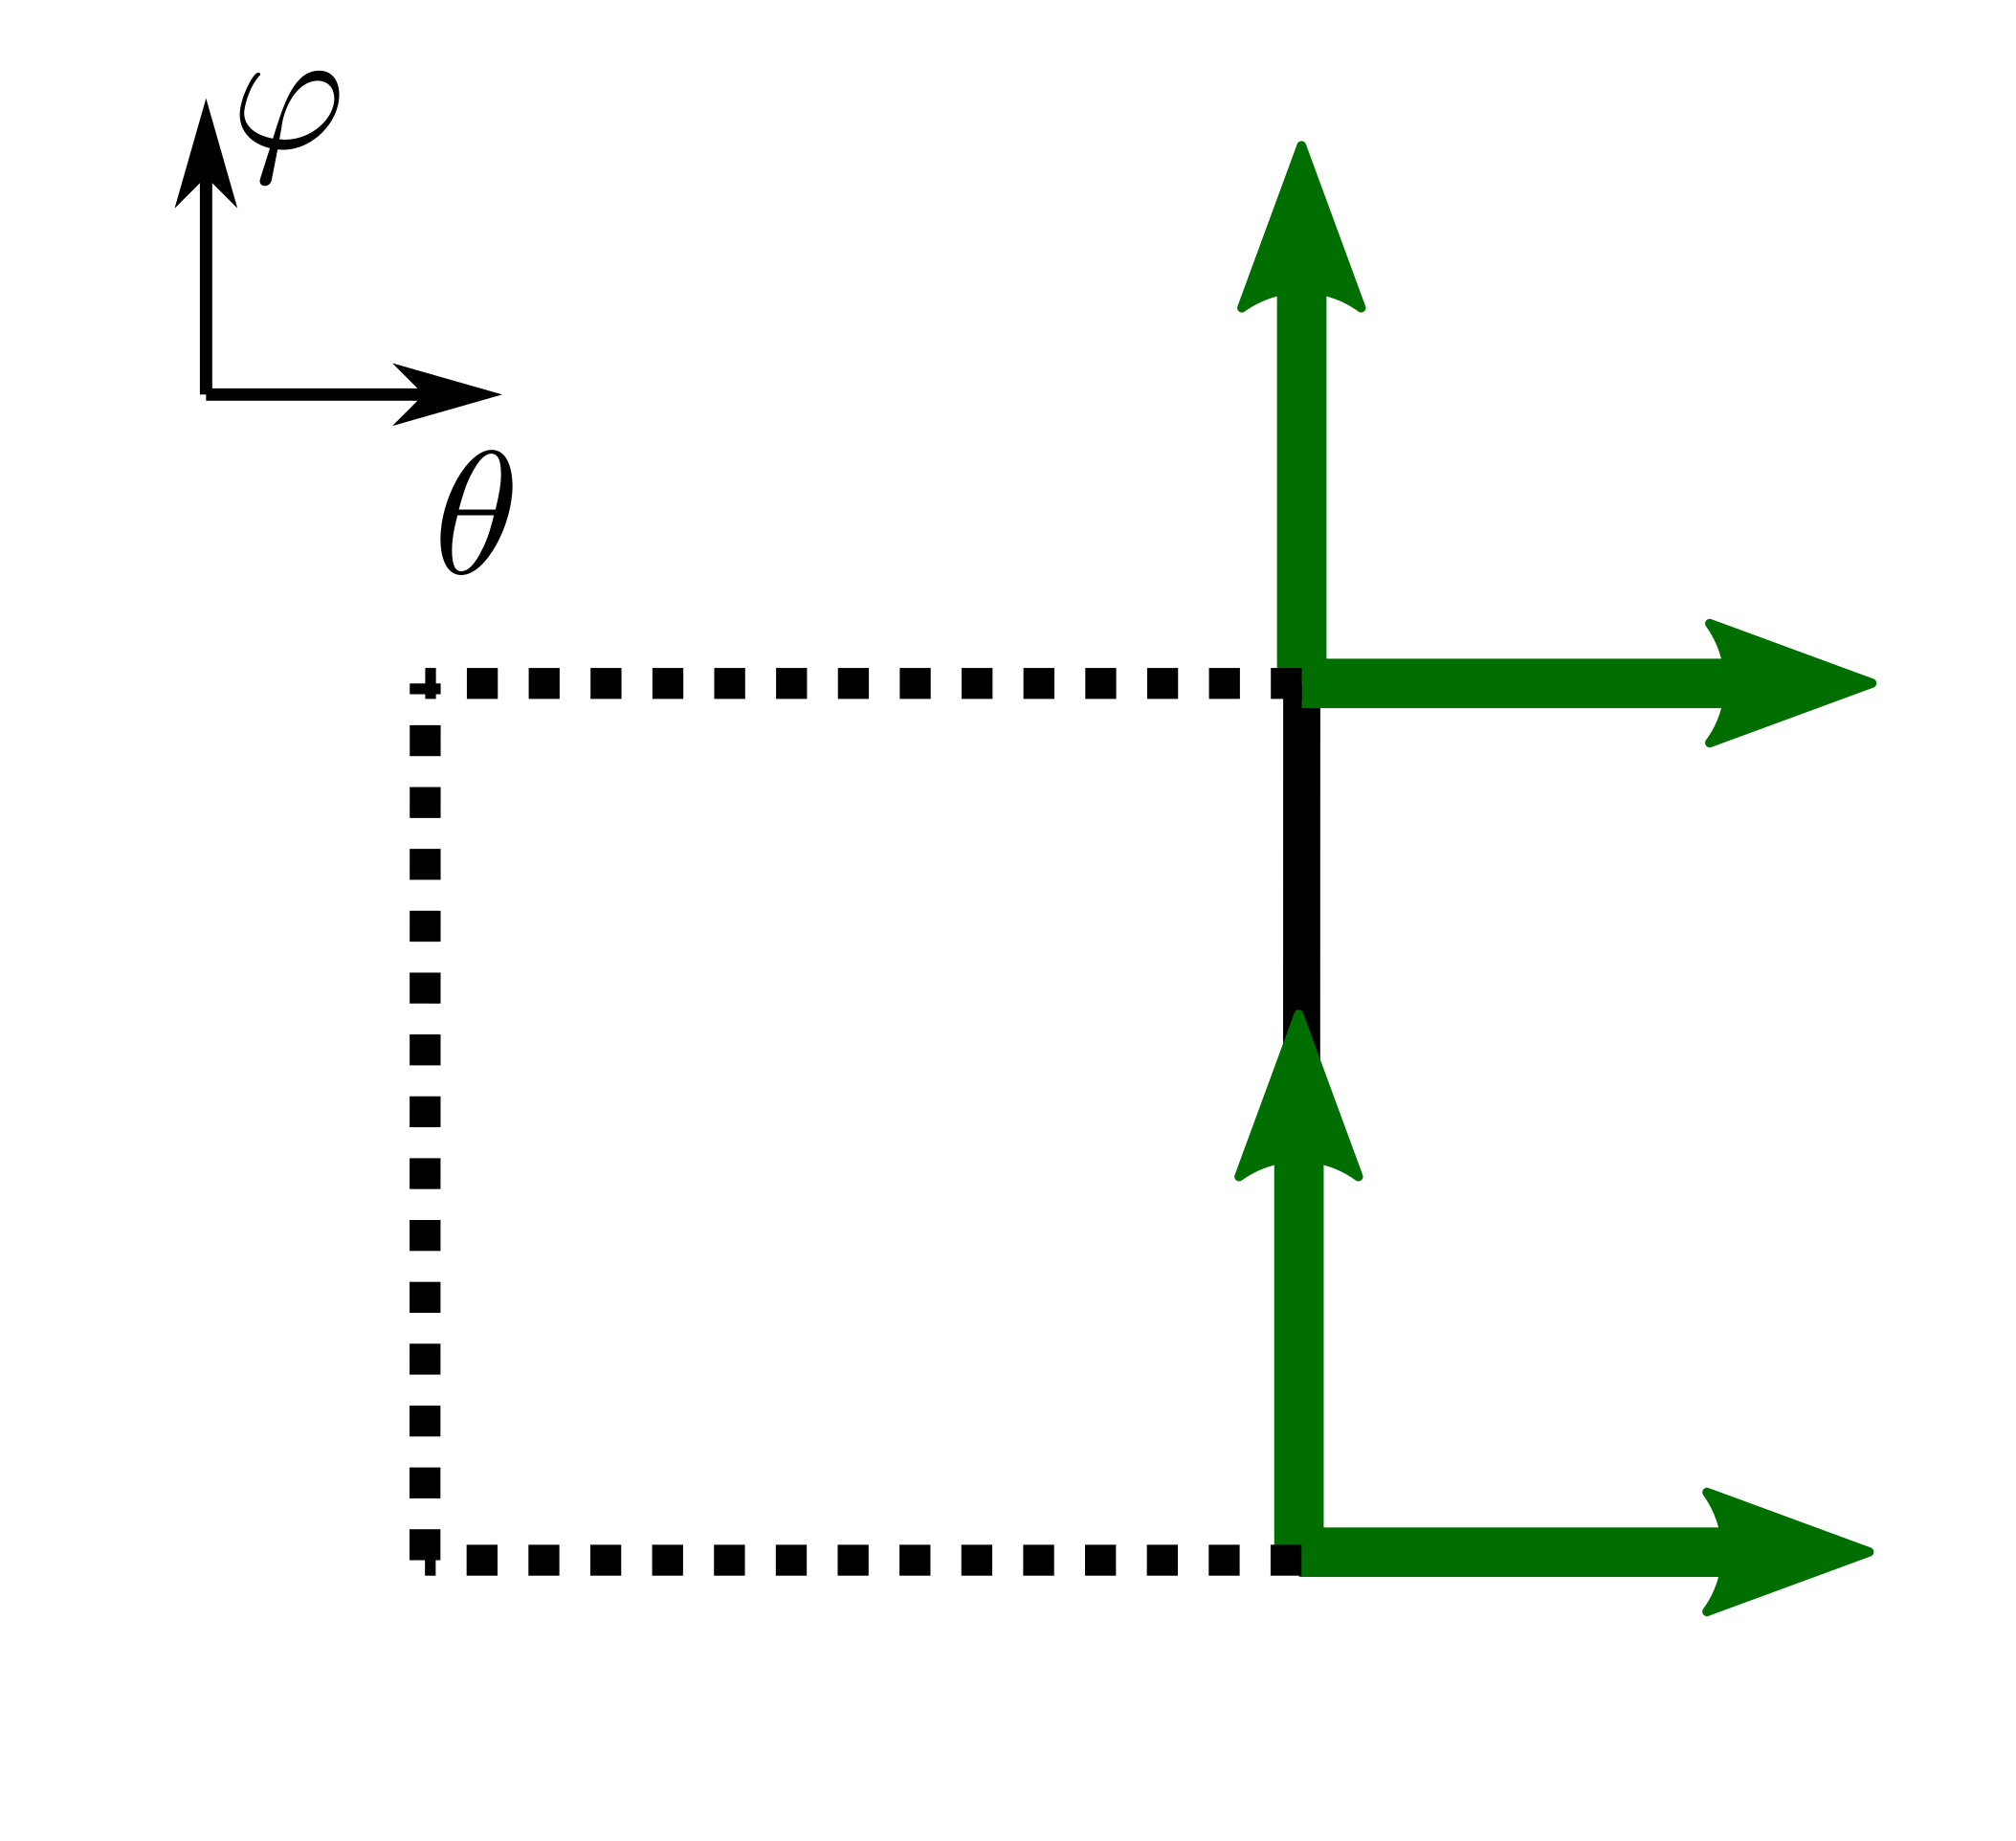
\includegraphics[width=\textwidth]{schemes/Gunter2D.png}
		\caption{ Gradients for the $\theta$-flux in the electrostatic setting }
		\label{fig:Gunter2D} 
	\end{subfigure}
	\begin{subfigure}[t]{0.32\textwidth}
		\centering
		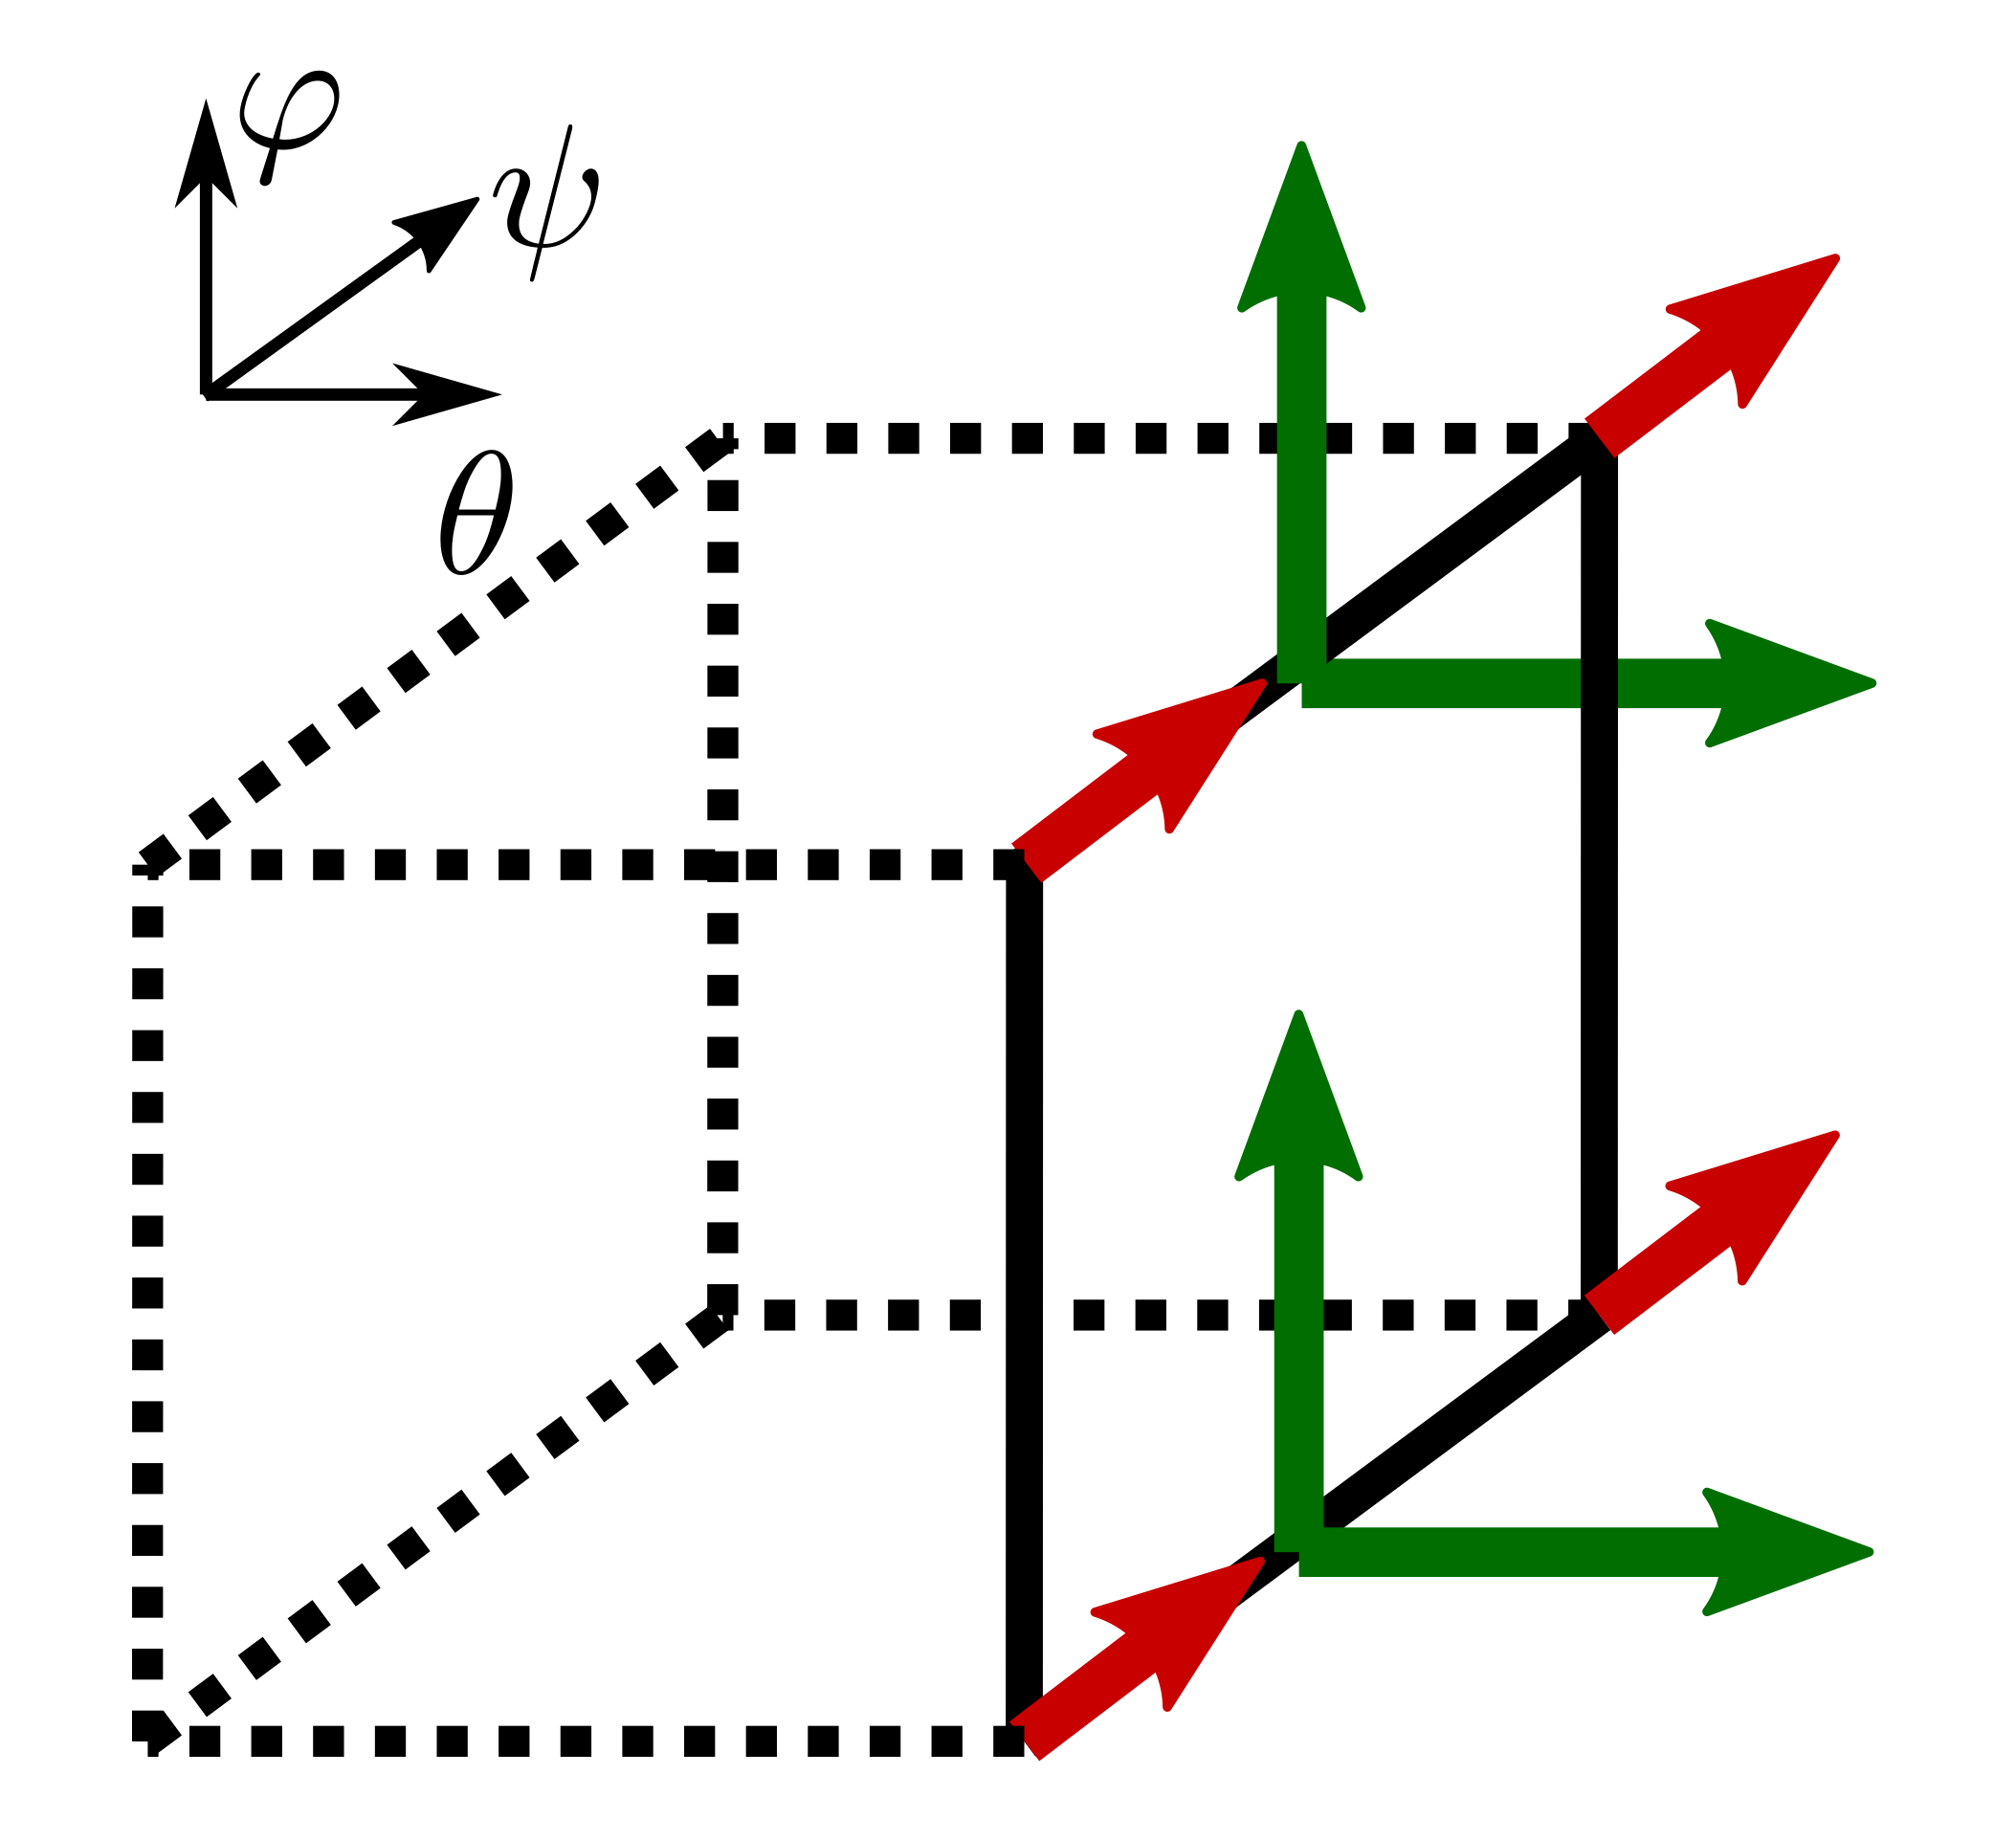
\includegraphics[width=\textwidth]{schemes/Gunter3D_theta.png}
		\caption{ Gradients for the $\theta$-flux in the electromagnetic setting   }
		\label{fig:Gunter3D_theta} 
	\end{subfigure}
	\begin{subfigure}[t]{0.32\textwidth}
		\centering
		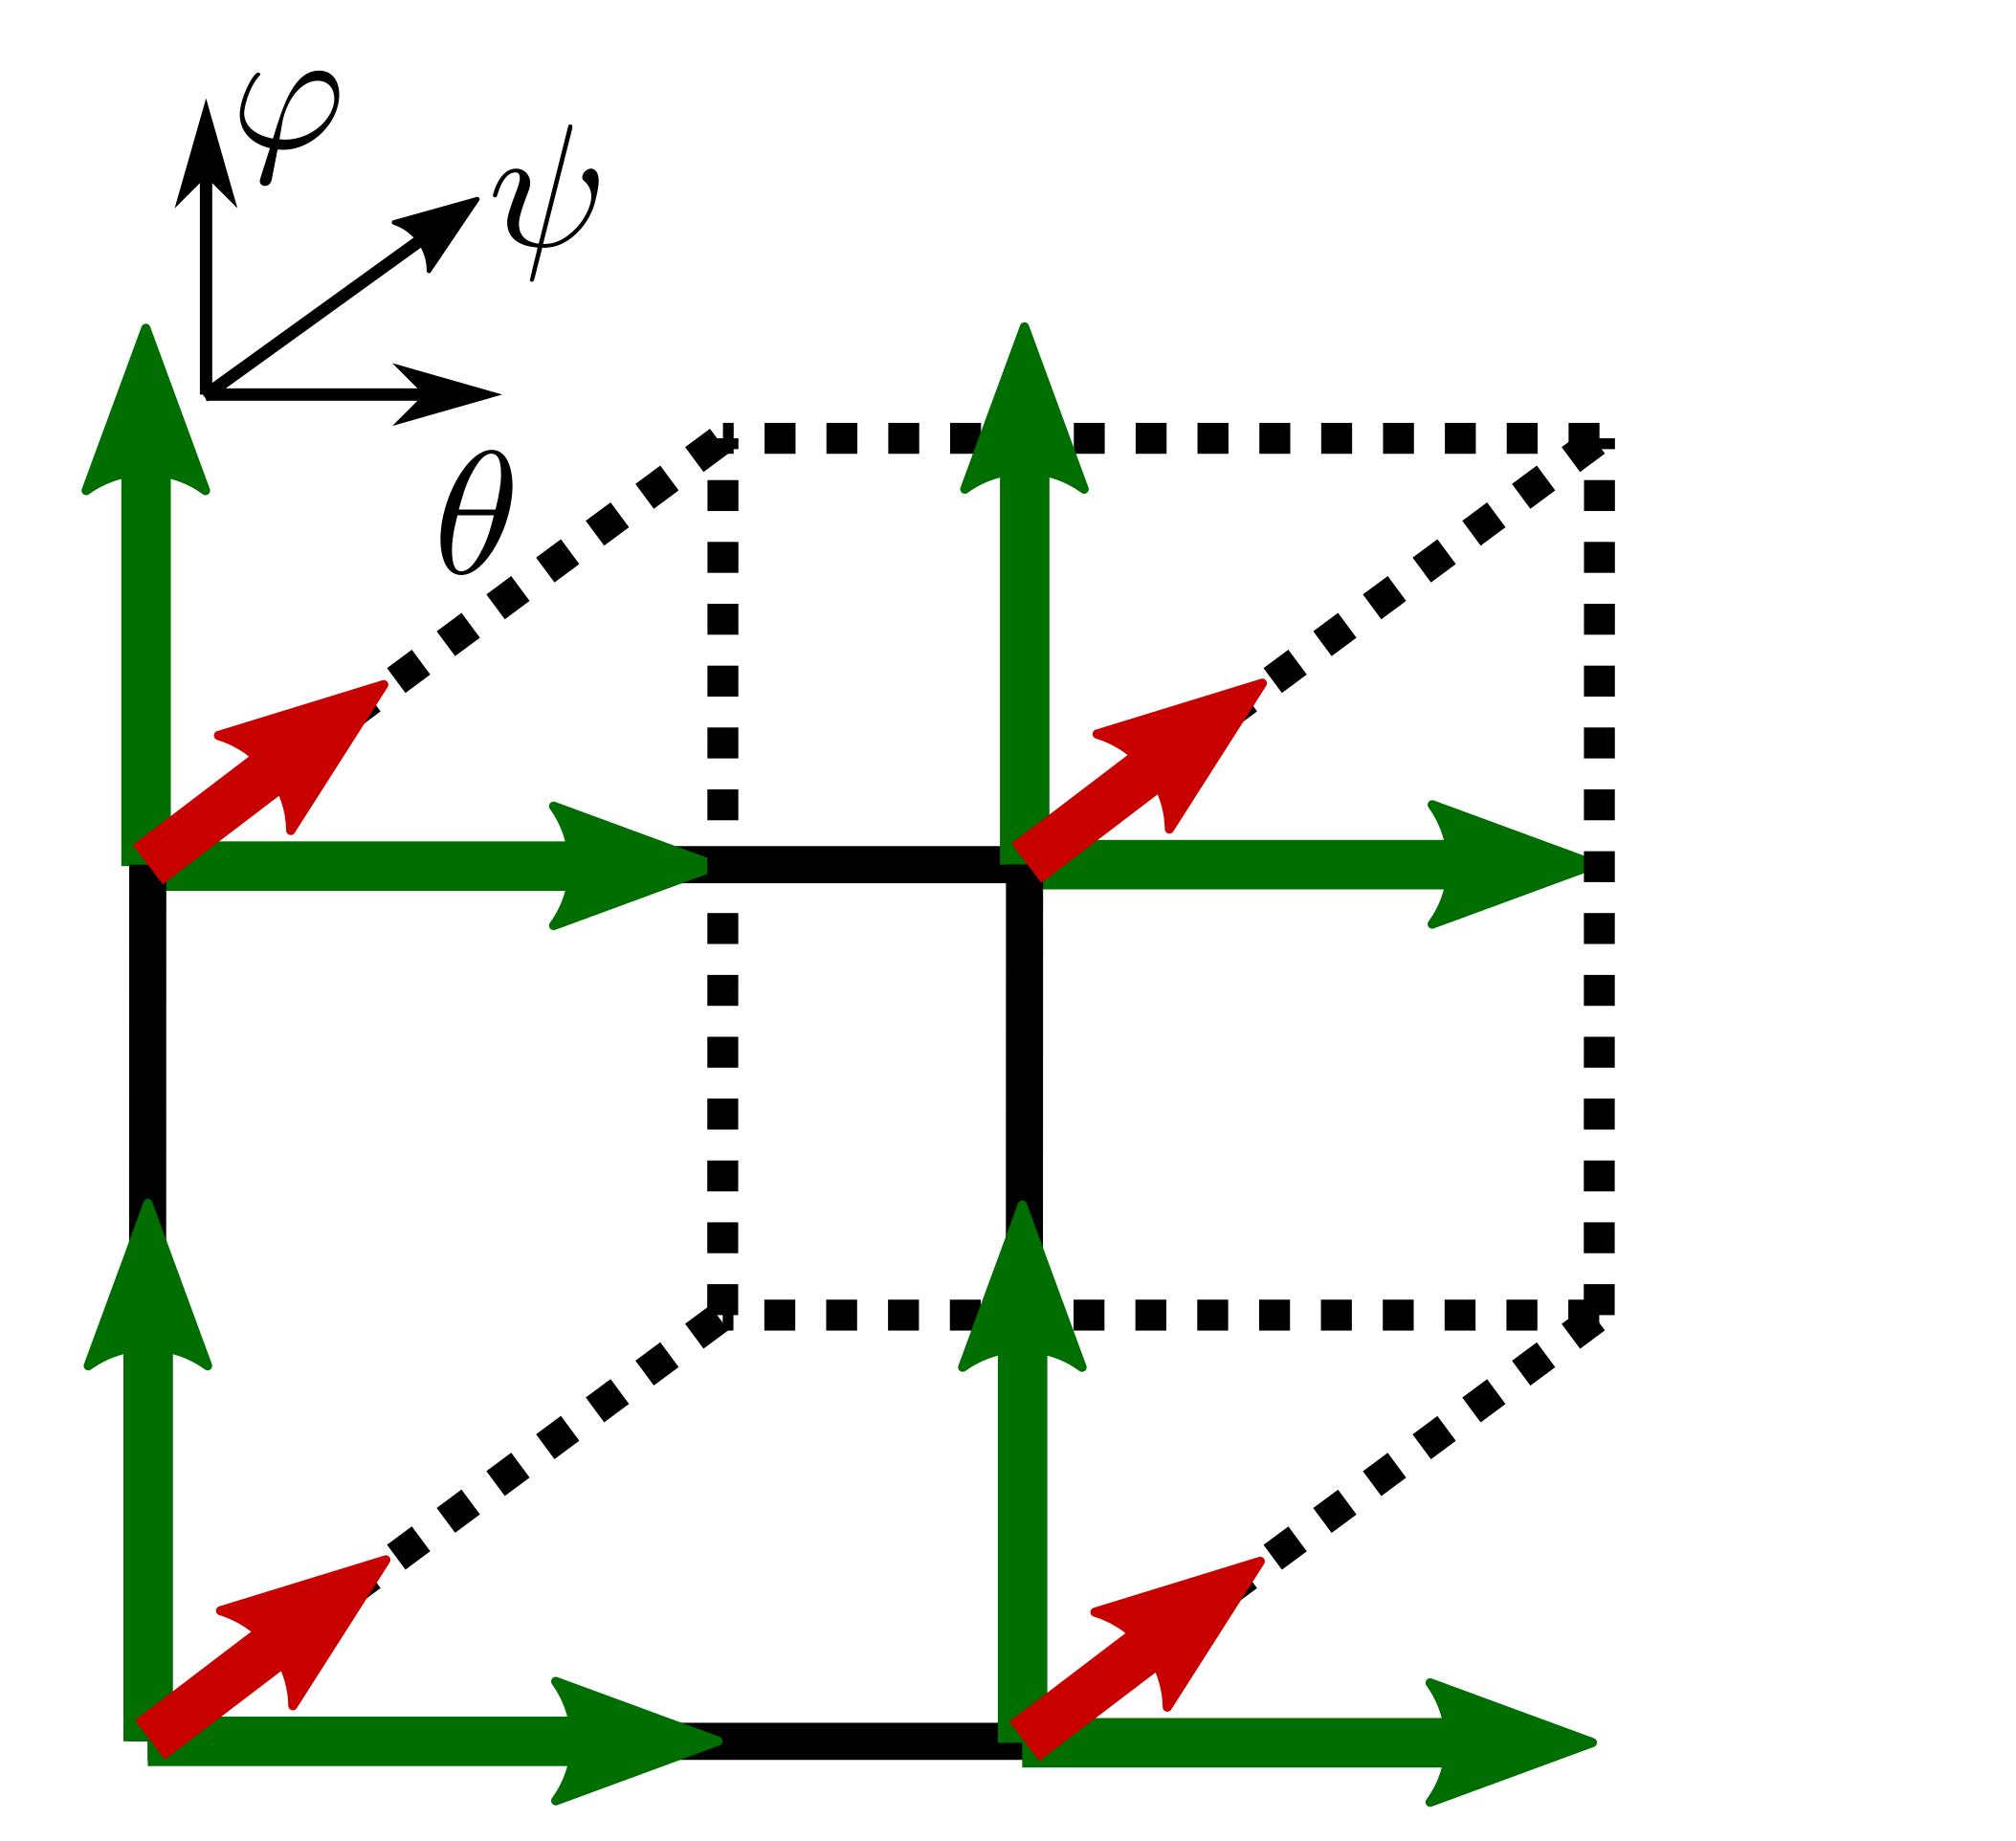
\includegraphics[width=\textwidth]{schemes/Gunter3D_psi.png}
		\caption{ Gradients for the $\psi$-flux in the electromagnetic setting   }
		\label{fig:GunterD_psi}
	\end{subfigure}
	\caption{Sketches showing the calculation of gradients for the parallel diffusion scheme. It shows the position where the different gradients are calculated that are relevant for a flux across the cell face with a solid line. Green and red arrows symbolize gradients in the equilibrium and in the radial direction, respectively.}
	\label{fig:GunterStencils_flutter}
\end{figure}


\subsection{Electromagnetic vorticity system}

The newly introduced fields $j_\parallel$ and $A_\parallel$ are solved implicitly along with the electric potential $\Phi$. As we face a coupled system that connects all points in the domain, direct solvers such as PASTIX are not suitable, especially for fine 3D meshes. We instead prefer to use iterative solvers available in the the PETSc or HYPRE libraries. For the original vorticity system, the Stabilized version of the Biconjugate Gradient method (BiCGStab) along with the Geometric Algebraic Multigrid (GAMG) preconditionner proved to be very efficient and it is desirable to use them on the new systems. This section describes some special numerical features in the construction of the system to facilitate the convergence of the above iterative scheme. \autoref{ssec:equilibrationBLockMatrices} introduces specific row and column scaling to equilibrate the blocks in the new system and \autoref{ssec:StaggeredFieldsMatrix} describes how to handle staggered fields to be compatible with the iterative scheme.

\subsubsection{Expression for the coupled system}

With the values for $n_e$ and $T_e$ known at time-step $n+1$, the vorticity equation (Eq. \ref{eq:VorticityEquation}) corresponds to a 3D costly system involving $\Phi$, $j_\parallel$, and $A_\parallel$. To solve it efficiently, the $j_\parallel$ advection and perpendicular diffusion are treated explicitly, allowing the integration of Ohm's law into the vorticity equation and Ampère's law. Then, at time-step $n+1$, the following dimensionless system coupling the two potentials $\Phi$ and $A_\parallel$ must be solved: \newline

\begin{align}
	\begin{pmatrix}
		\label{eq:implicitSytem}
		\nabla \cdot \left[ D_\perp \nabla_\perp \circ \right] + \nabla \cdot \left[ D_\parallel \nabla_\parallel \circ \mathbf{b} \right] & 
		\frac{\beta_0}{\delta t} \nabla \cdot \left[ D_\parallel \circ \mathbf{b} \right] \\
		D_\parallel \nabla_\parallel \circ &
		\frac{\beta_0}{\delta t} D_\parallel \circ - \nabla \cdot \left[ \nabla_\perp \circ \right]
	\end{pmatrix}
	\begin{pmatrix}
		\Phi^{n+1} \\ A_\parallel^{n+1}
	\end{pmatrix} 
	= \nonumber \\
	\begin{pmatrix}
		\nabla \cdot \left[ D_t j^{n}_\parallel \mathbf{b} \right] + \text{RHS}^\Phi \\
		D_t j^{n}_\parallel + \text{RHS}^{A_\parallel}
	\end{pmatrix}
\end{align}

with $D_\perp = \frac{m_i n_i}{B^2 \delta_t}$, $D_\parallel = \frac{1}{\eta_\parallel + \mu}$, $D_t = \frac{\mu}{\eta_\parallel + \mu}$, and $\mu = m_e / (m_u n_e \delta_t)$ accounting for electron inertia effects. The parameter $\delta t$ derives from the integration scheme and is equal to the time-step in the case of a first-order implicit Euler scheme. \newline

Since $\eta_\parallel \propto T_e^{-1.5}$, the parallel resistivity $\eta_\parallel$ is often a small parameter that leads to strong anisotropy between the perpendicular and parallel Laplacian operators. However, the electron inertia term, being implemented in the current solver, acts as an upper limit for the parallel diffusion coefficient, which is expected to improve the matrix conditioning as $\eta_\parallel$ approaches zero. This is in contrast to the original electrostatic model from \cite{Bufferand2021}. \newline


\subsubsection{Equilibration of the Matrix Blocks}
\label{ssec:equilibrationBLockMatrices}
The matrices in the electromagnetic model \autoref{sec:DedimensionalizedElectromagneticModelS3X} can be decomposed in 2x2 or 3x3 block matrices that apply on the respective fields $\Phi$, $A_\parallel$ and/or $j_\parallel$. Apart of the use of dedimensionalized quantities, no effort was made so far to ensure that the blocks are roughly of the same order of the magnitude, which is important for the condition number of the matrix, nor that the matrix is diagonally dominant, which is generally a desirable feature for fast convergence of iterative schemes. \\
In the following bits, we introduce some column $c_X$ and row $r_X$ scaling factors that are specific to the blocks $X$ of the matrix such that the above conditions are fullfilled as well as possible. To ensure a correct solution, the row scaling factor $r_X$ must be applied to the corresponding entry in the RHS vector and as a matter of fact, in the original vorticity matrix, we already have $r_\Phi = J$ the metrical Jacobian from \autoref{ssec:MetricCurvilinearCoordinates} to remove the effect of different mesh sizes in the domain on the discrete Laplacian operators. The column scaling factors $c_X$ must be taken care of when retrieving the fields from the numerical solution and it is strongly recommended to apply them to the initial guess for the iterative scheme. \\ 
Some exisiting algorithms optimize the scaling task such as ---cite---. However, they all require an expensive matrix analysis phase that must be repeated regularly since the matrix changes with the progress of the simulation. Therefore, we use the knowledge about the construction of the matrix blocks to define sufficiently good scaling factors. \\
In the system with electron inertia \autoref{eq:vorticityEquation_Elect	ronInertia_dedimensionalized_matrix}


\subsubsection{Staggered Fields in the Matrix}
\label{ssec:StaggeredFieldsMatrix}
The GAMG multigrid solves the system on different coarser levels by restricting the matrix and the RHS vector and then interpolates the solution back to the finer levels. In the new system, two consecutive entries belong to different fields, which makes the whole restriction-interpolation task obsolete from the very first level since neither the solution nor the matrix entries are similar between neighbours. In general, PETSc takes care of multiple fields in a coupled system if one defines a block size (in our case either 2 or 3) that indicates GAMG how to match corresponding entries.vim  However, as seen in \autoref{ssec:SpatialDiscretization}, the fields $A_\parallel$ and $j_\parallel$ are defined on a staggered grid in poloidal and toroidal directions as opposed to the centered field for $\Phi$. For the system it means that at each wall in negative directions (at the left target and for non-axisymmetric geometries), a line and column for $\Phi$ exists but not for the two other fields. This in turn is problematic for GAMG as the blocks are globally defined and two different fields would again end up together and the total system size might even not be a multiple of the blocksize (2 resp. 3), which at all prevents the initialization of the preconditioner. \\


For the parallel diffusion on the electric potential $\nabla \cdot \left[ D_\parallel \nabla_\parallel \Phi \mathbf{b} \right]$ with flutter, we do not use the stencil introduced in Sec. \ref{ssec:3DGunter}. To avoid numerical difficulties and the appearance of unphysical modes, the discretization of this term needs to be consistent with the parallel gradient and divergence operators in the same system. Since the grid for $A_\parallel$ and $j_\parallel$ is only staggered in the $\theta$ and $\varphi$ directions, we do not know them in the radial corners from Figs. \ref{fig:Gunter3D_theta} and \ref{fig:GunterD_psi}. Instead, the discrete diffusion operator is defined as the combination of the operators for the gradient and the divergence. It involves two neighbors on both radial sides, so the resulting stencil is less compact but consistent with the remaining system. Note that in cases without flutter ($b^\psi = 0$), the diffusion operator exactly corresponds to Günter's scheme \cite{gunter2005} because the staggered fields are known at the position of the green gradients in Fig. \ref{fig:GunterStencils_flutter}. \newline


